\documentclass[12pt, a4paper]{book}
\begin{document}
\chapter{Model independent approach}\label{chap:Best_ML_MI}
The results for the network optimizations can be seen in Appendix \ref{chap:network_opt}, where it became apparent that the performance of BDTs is better at scoring a higher significance than NNs, and faster. Because of this and time constraints of this thesis 
we decided to compute the results of the model dependent and model independent search using BDTs only. \\\\
In this chapter we will explore how three BDTs fare at learning the six models we have. These three BDTs were trained on a dataset containing 80\% of all SM background events and 80\% of all our signal events in orthogonal Signal Regions (SR). To recap the regions we have
\begin{itemize}
   \item SR1: $m_{ll} >110$ GeV and $E_T^{miss} \in [50, 100]$ GeV
   \item SR2: $m_{ll} >110$ GeV and $E_T^{miss} \in [100, 150]$ GeV
   \item SR3: $m_{ll} >110$ GeV and $E_T^{miss} >150$ GeV
\end{itemize}
To compare this method to the previous method we will statistically combine the mass exclusions results for each SR for each final state in a model. To navigate through the process we will again take a model as an example, the Dark Higgs Heavy Dark Sector model, 
and afterwards present the combined exclusion limits for every model. All the results can be found in the GitHub repo\footnote{Available here: \href{https://github.com/rubenguevara/Master-Thesis/tree/master/Plots/XGBoost/Model_independent}{https://github.com/rubenguevara/Master-Thesis/tree/master/Plots\\/XGBoost/Model\_independent}}. 

\clearpage
\graphicspath{{../../../Plots/}}
\section{Walkthrough of method}
Following the same method presented in Chapter \ref{sec:Walkthrough}. We start by looking at the feature importance of the network trained on SRs, this can be seen in Figure \ref{fig:DH_HDS_feat_SRs} where we show the feature importance using the \textit{weight}\footnote{See Chapter \ref{sec:feat} for definition} metric to not overflow the chapter. 
From these results we see that as hoped, \textbf{Question: can i say as hoped if I havent earlier explicitly said I hope this?} the variables that are of importance change in every region. Even though they change, they are all are the ones we expect from a dilepton and MET final state.\\
\begin{figure}[!ht]
	\centering
	\begin{subfigure}[b]{0.7\textwidth}
      \centering
      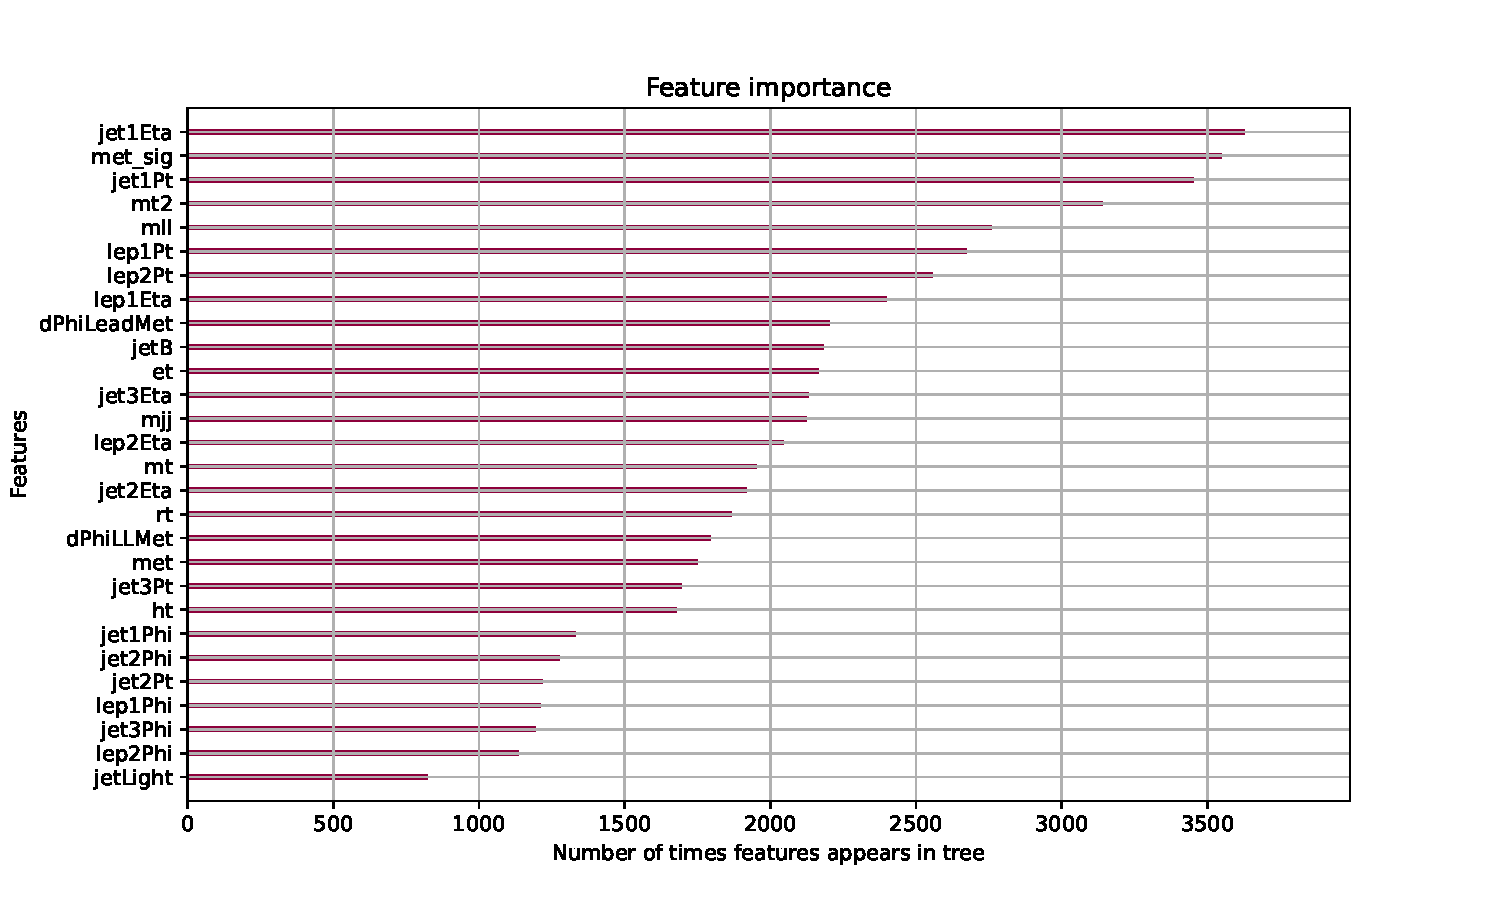
\includegraphics[width=1\textwidth]{XGBoost/Model_independent/50-100/feature_importance/weight.pdf}\caption{Network trained in SR1}
      \end{subfigure}
      \hfill
      \begin{subfigure}[b]{0.7\textwidth}
         \centering
         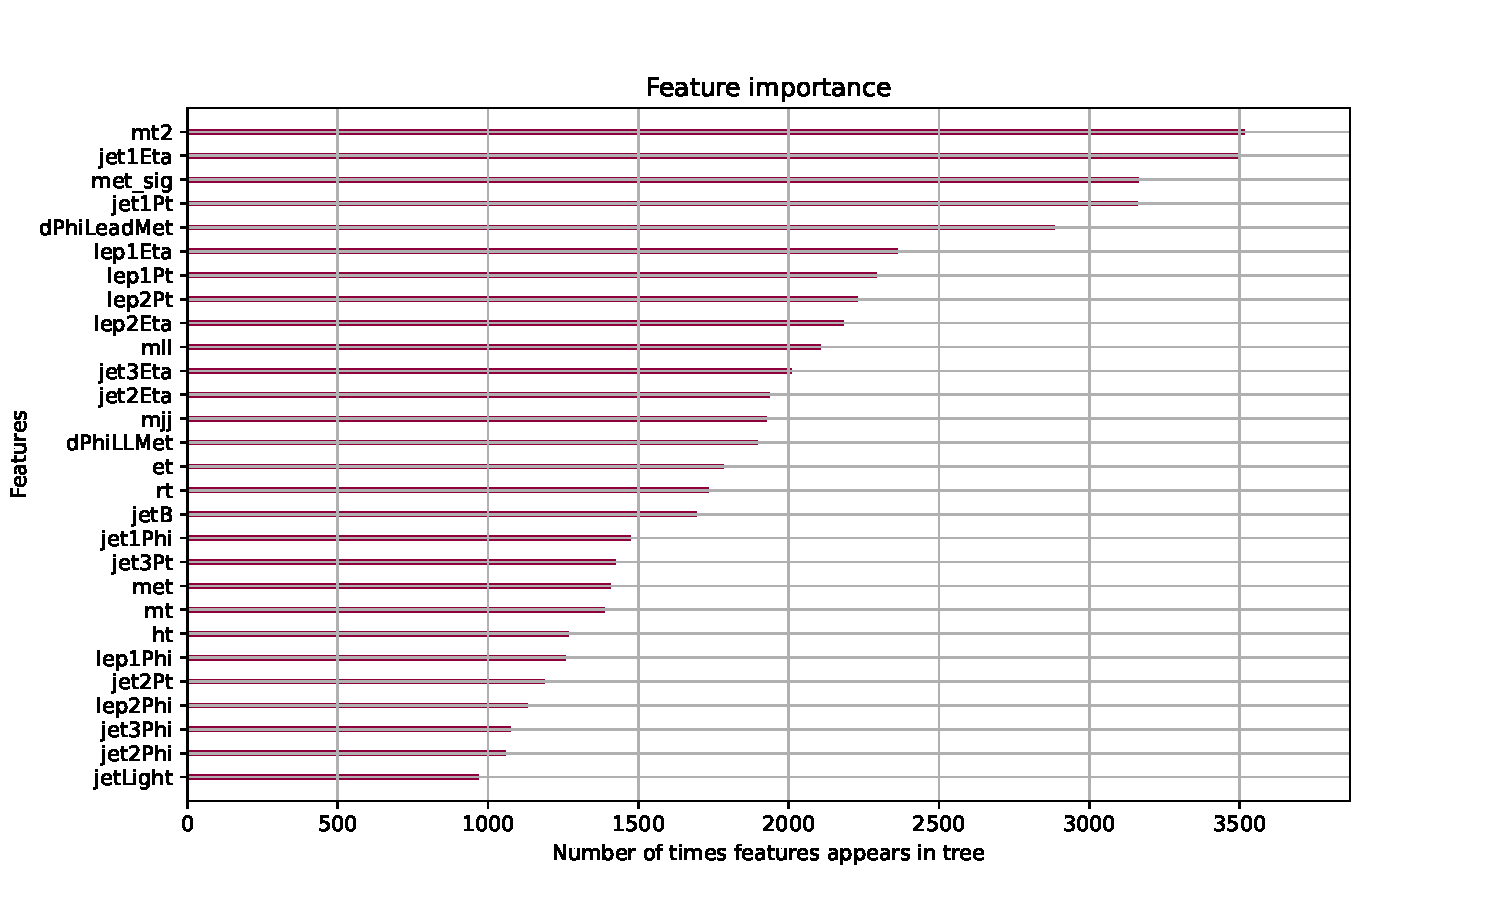
\includegraphics[width=1\textwidth]{XGBoost/Model_independent/100-150/feature_importance/weight.pdf}\caption{Network trained in SR2}
      \end{subfigure}
      \hfill
      \begin{subfigure}[b]{0.7\textwidth}
         \centering
         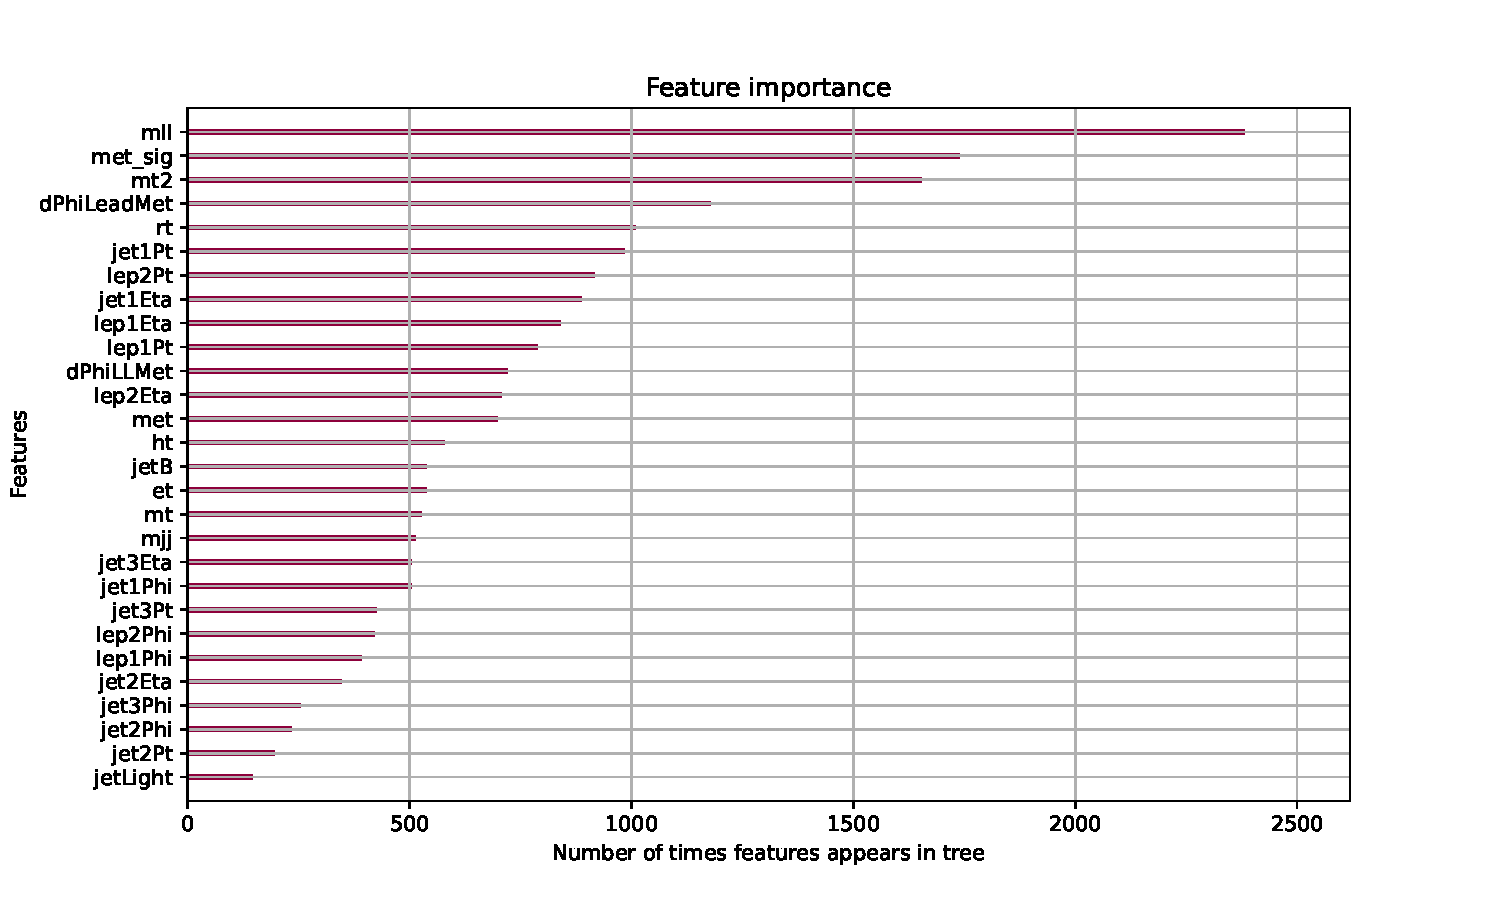
\includegraphics[width=1\textwidth]{XGBoost/Model_independent/150/feature_importance/weight.pdf}\caption{Network trained in SR3}
      \end{subfigure}
   \caption{Feature importance for network trained on Z' DH HDS in all SRs}\label{fig:DH_HDS_feat_SRs}
\end{figure}
\\This time however we decided to show the validation plots, ROC curve and expected significance for every signal region of the model together. This can be seen in Figure \ref{fig:DH_HDS_SR1}, \ref{fig:DH_HDS_SR2} and \ref{fig:DH_HDS_SR3} for SR1, SR2 and SR3 respectively. 
Here we can again see how having different SRs changes the performance of the network.\\
\begin{figure}[!ht]
	\centering
	\begin{subfigure}[b]{0.49\textwidth}
      \centering
      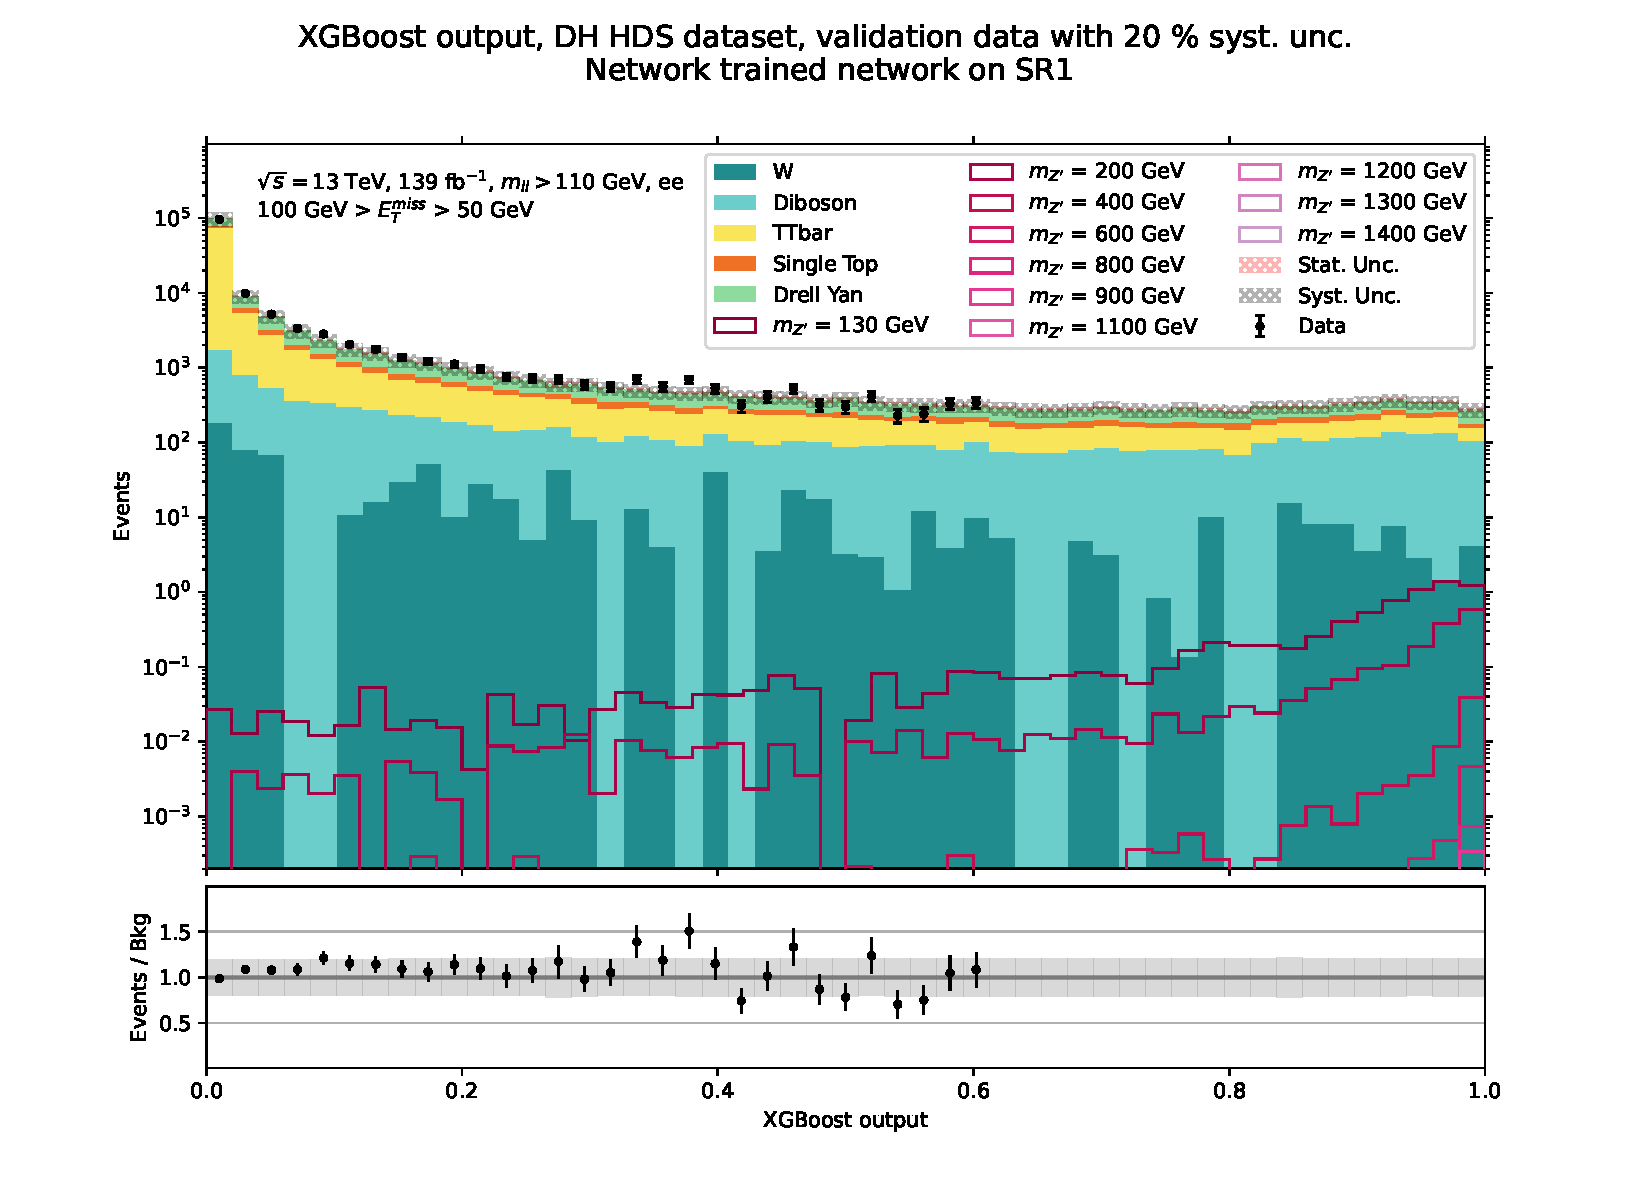
\includegraphics[width=1\textwidth]{XGBoost/Model_independent/50-100/DH_HDS/VAL_ee.pdf}
   \end{subfigure}
   \hfill
   \begin{subfigure}[b]{0.49\textwidth}
      \centering
      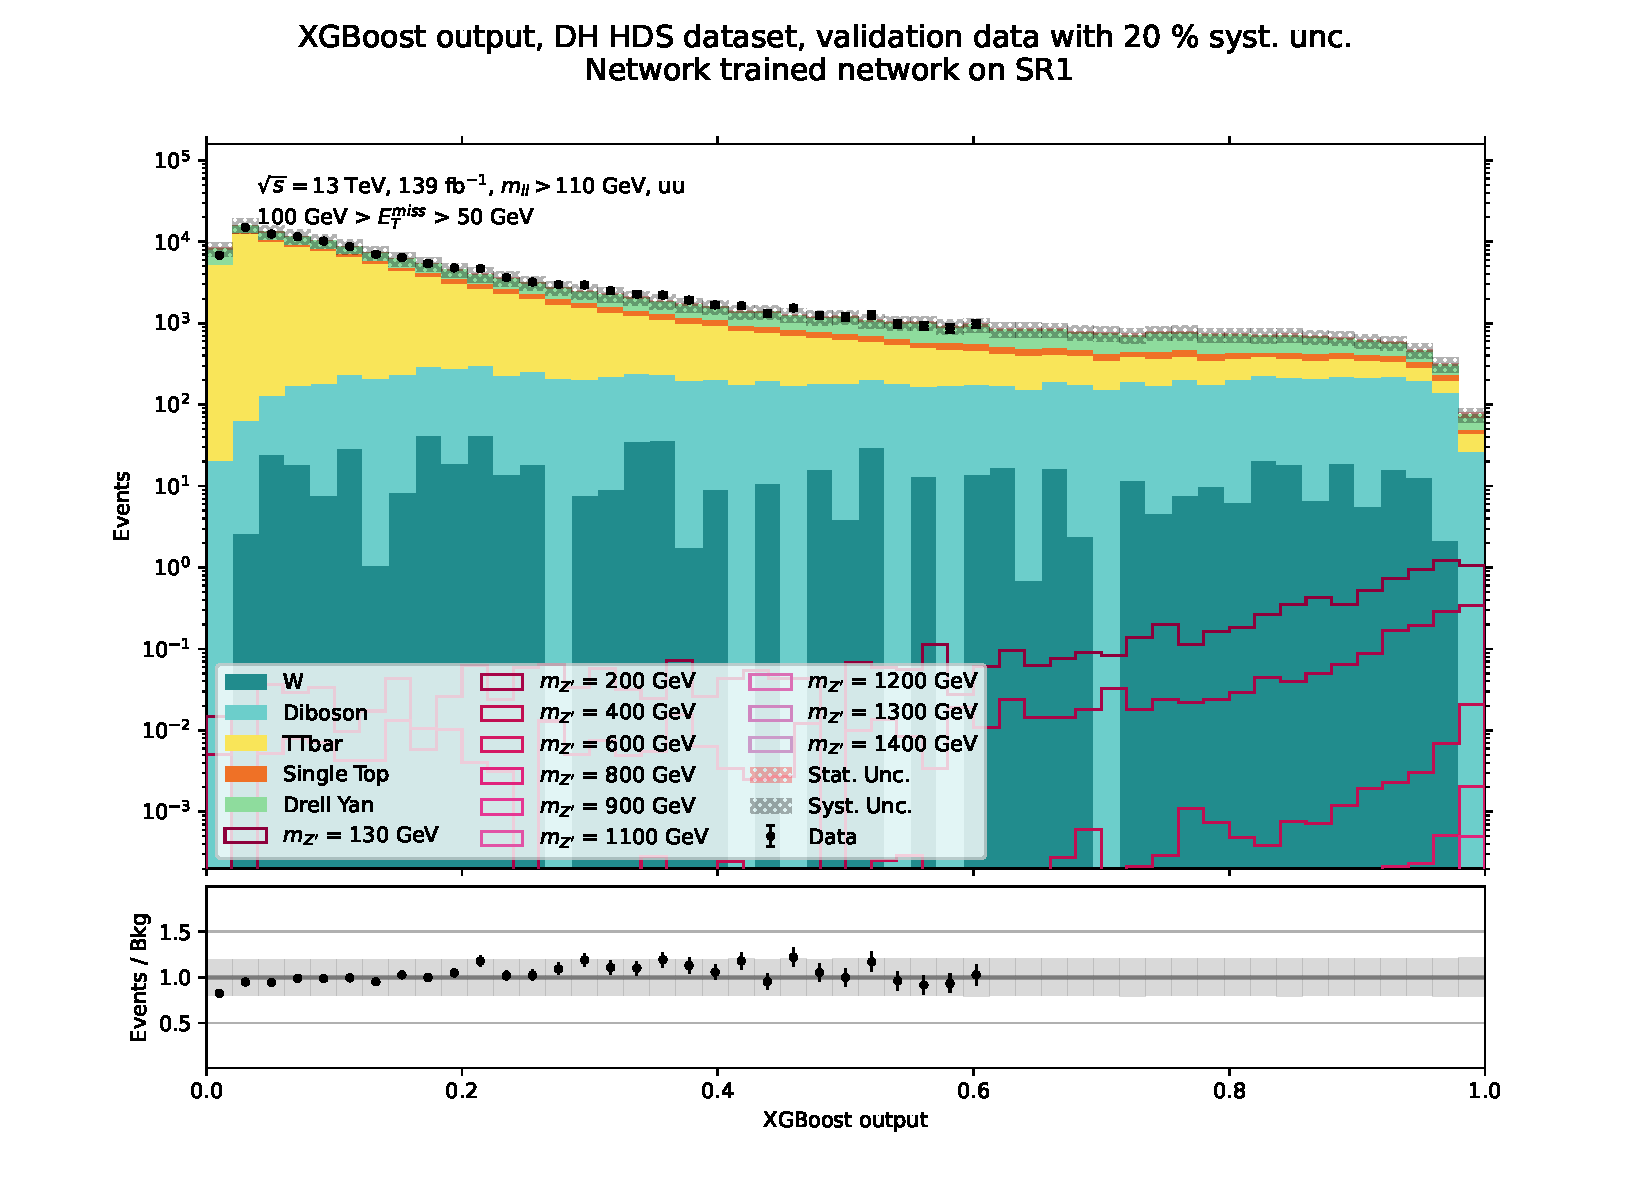
\includegraphics[width=1\textwidth]{XGBoost/Model_independent/50-100/DH_HDS/VAL_uu.pdf}
   \end{subfigure}
   \hfill
   \begin{subfigure}[b]{0.49\textwidth}
      \centering
      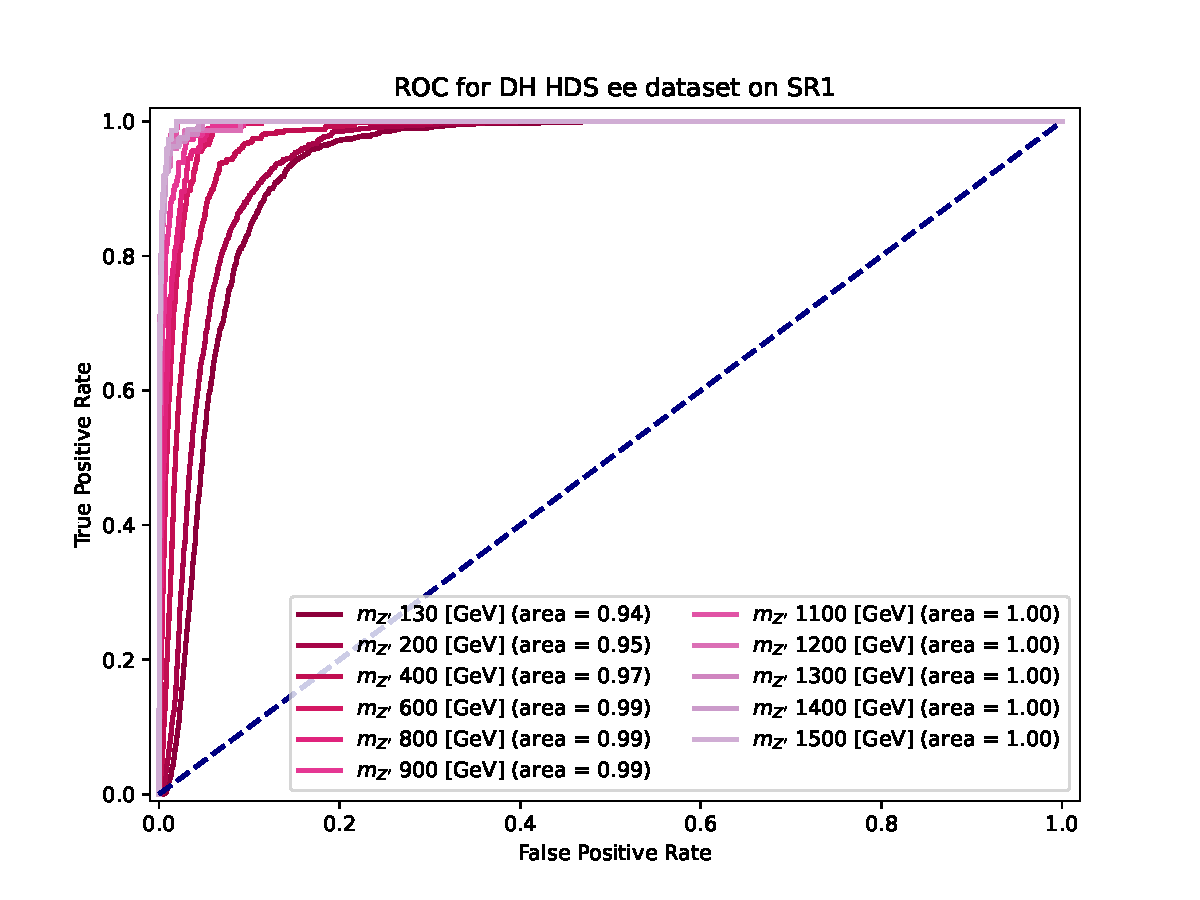
\includegraphics[width=1\textwidth]{XGBoost/Model_independent/50-100/DH_HDS/ROC_ee.pdf}
   \end{subfigure}
   \hfill
   \begin{subfigure}[b]{0.49\textwidth}
      \centering
      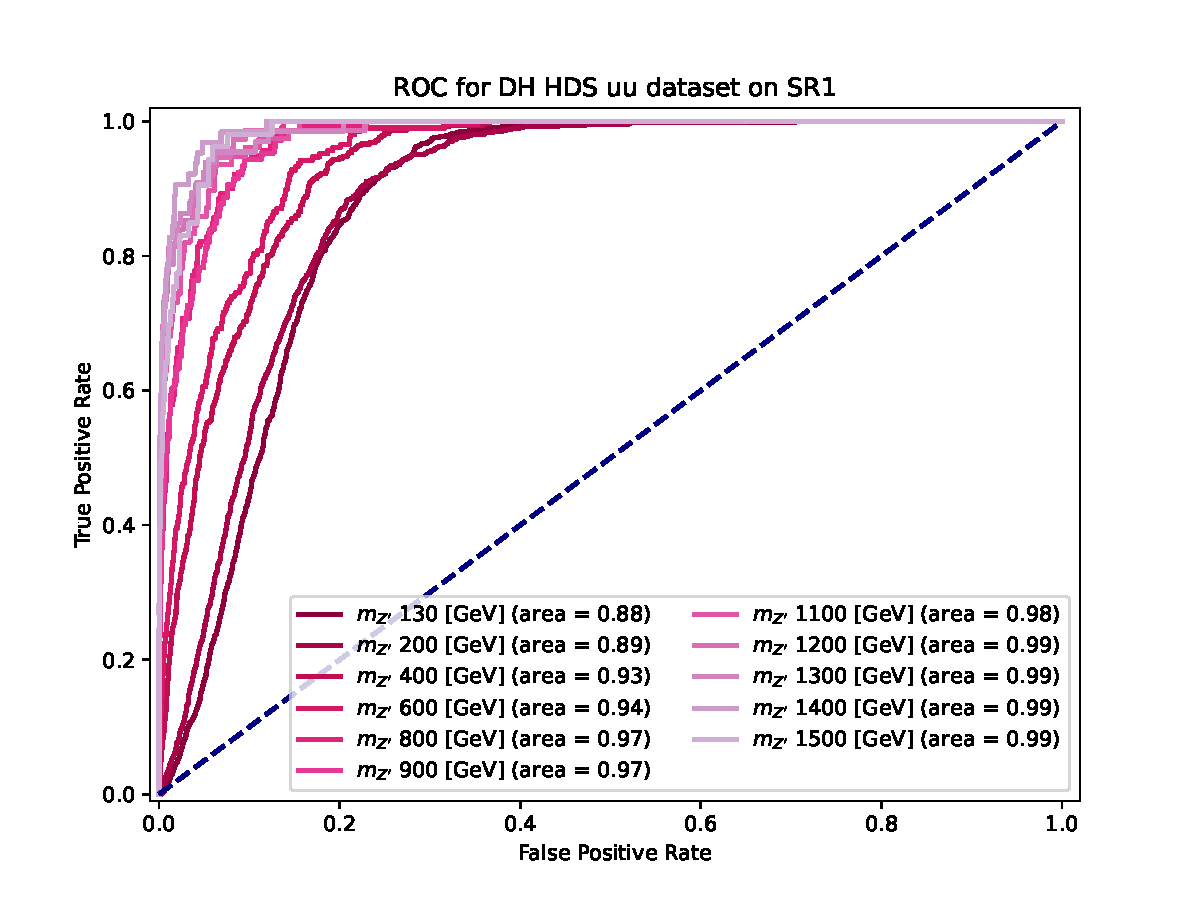
\includegraphics[width=1\textwidth]{XGBoost/Model_independent/50-100/DH_HDS/ROC_uu.pdf}
   \end{subfigure}
   \hfill
	\begin{subfigure}[b]{0.49\textwidth}
      \centering
      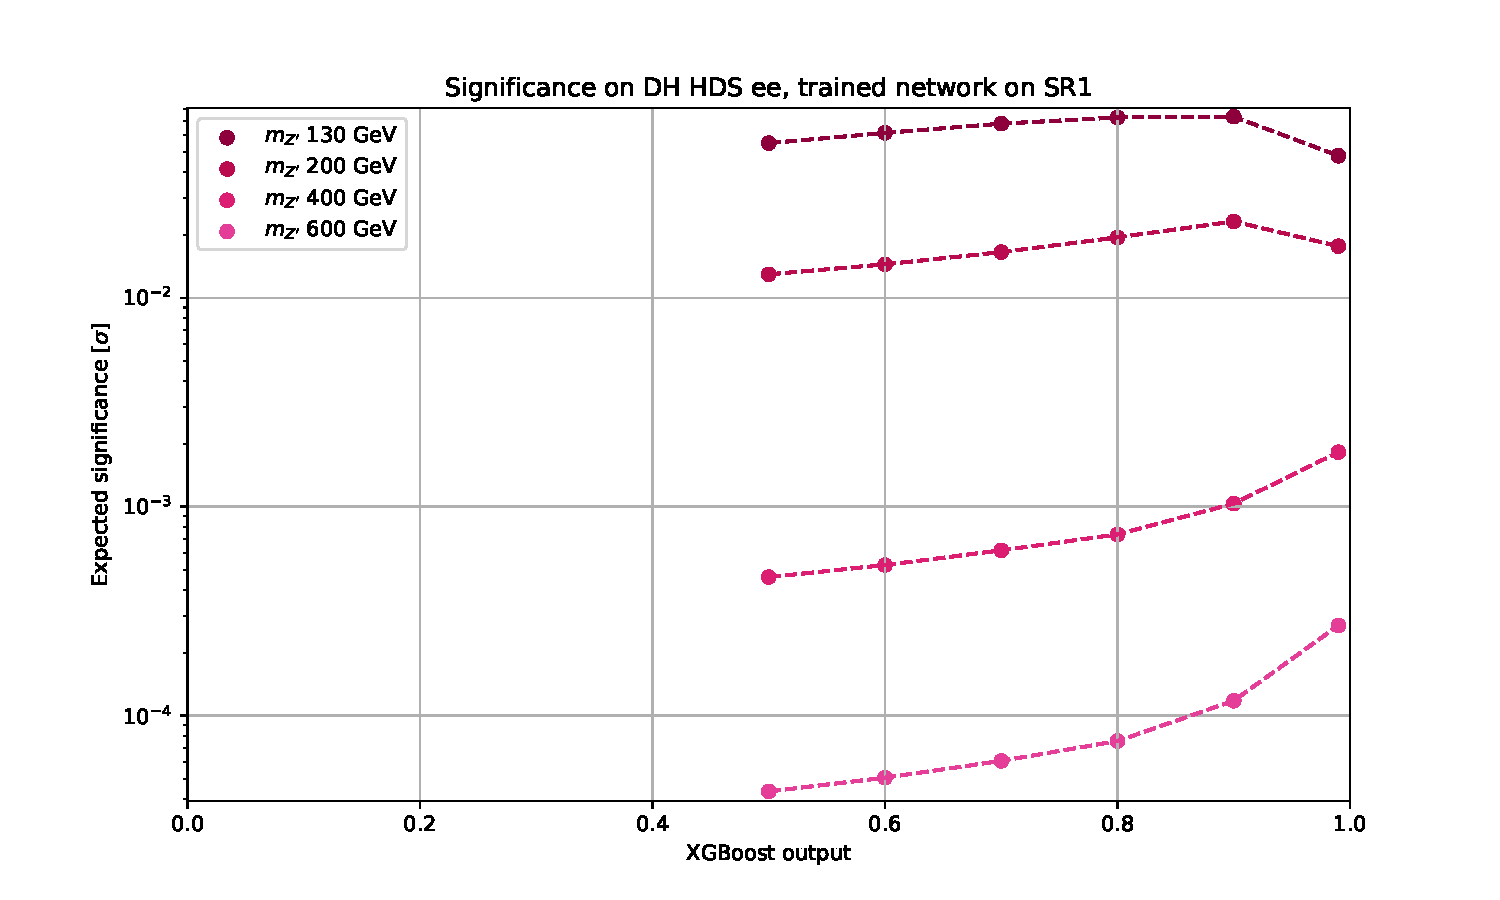
\includegraphics[width=1\textwidth]{XGBoost/Model_independent/50-100/DH_HDS/EXP_SIG_ee.pdf}
   \end{subfigure}
   \hfill
   \begin{subfigure}[b]{0.49\textwidth}
      \centering
      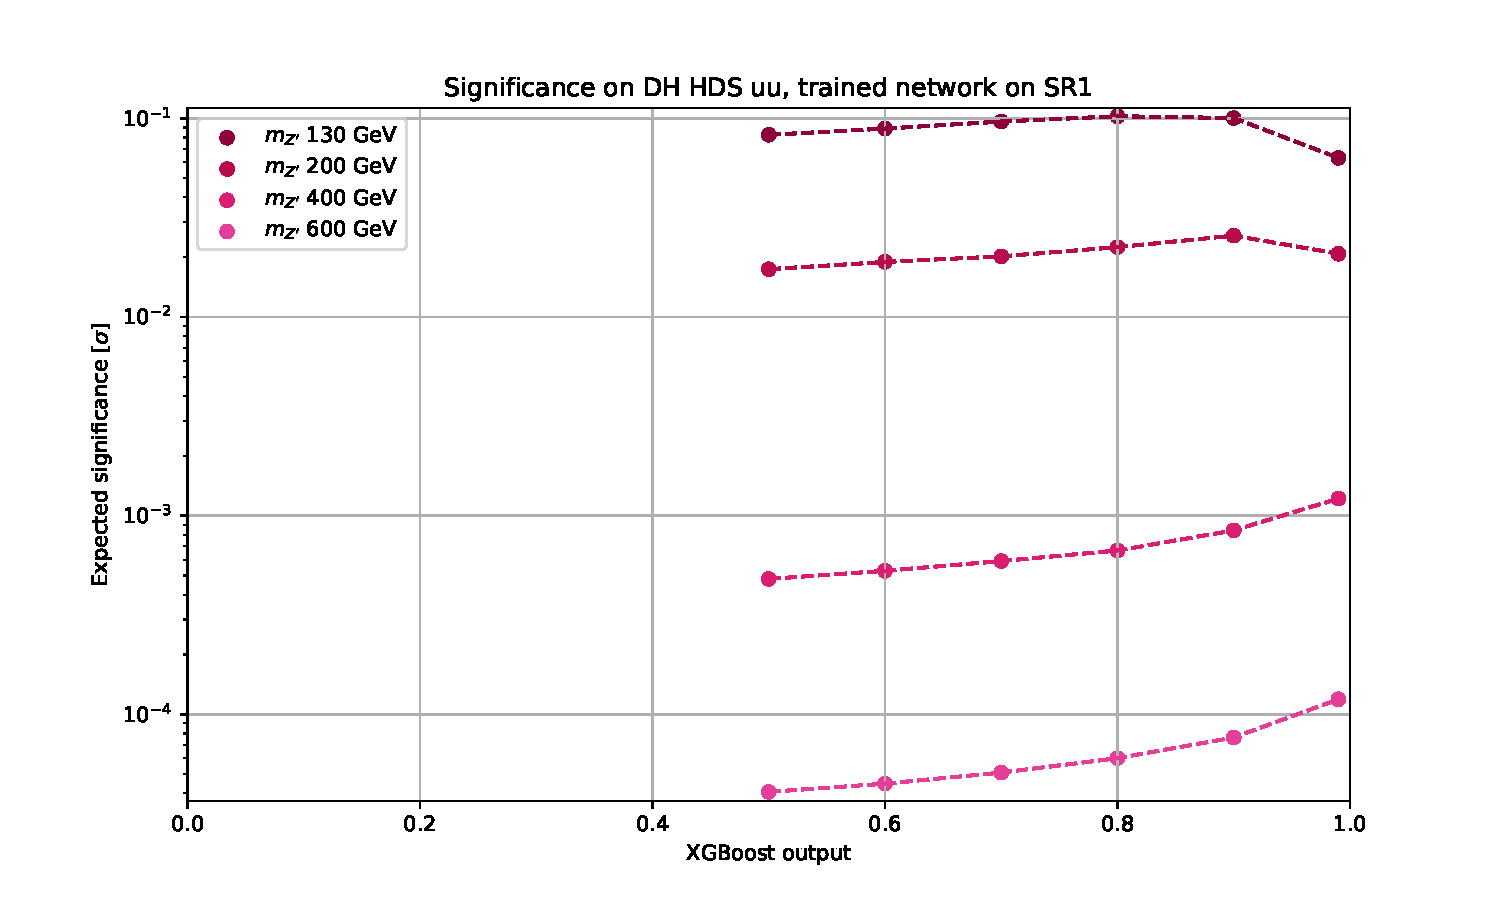
\includegraphics[width=1\textwidth]{XGBoost/Model_independent/50-100/DH_HDS/EXP_SIG_uu.pdf}
   \end{subfigure}
   \caption{XGBoost results for DH HDS model on $ee$ and $\mu\mu$ channel in SR1}\label{fig:DH_HDS_SR1}
\end{figure}
\begin{figure}[!ht]
	\centering
	\begin{subfigure}[b]{0.49\textwidth}
      \centering
      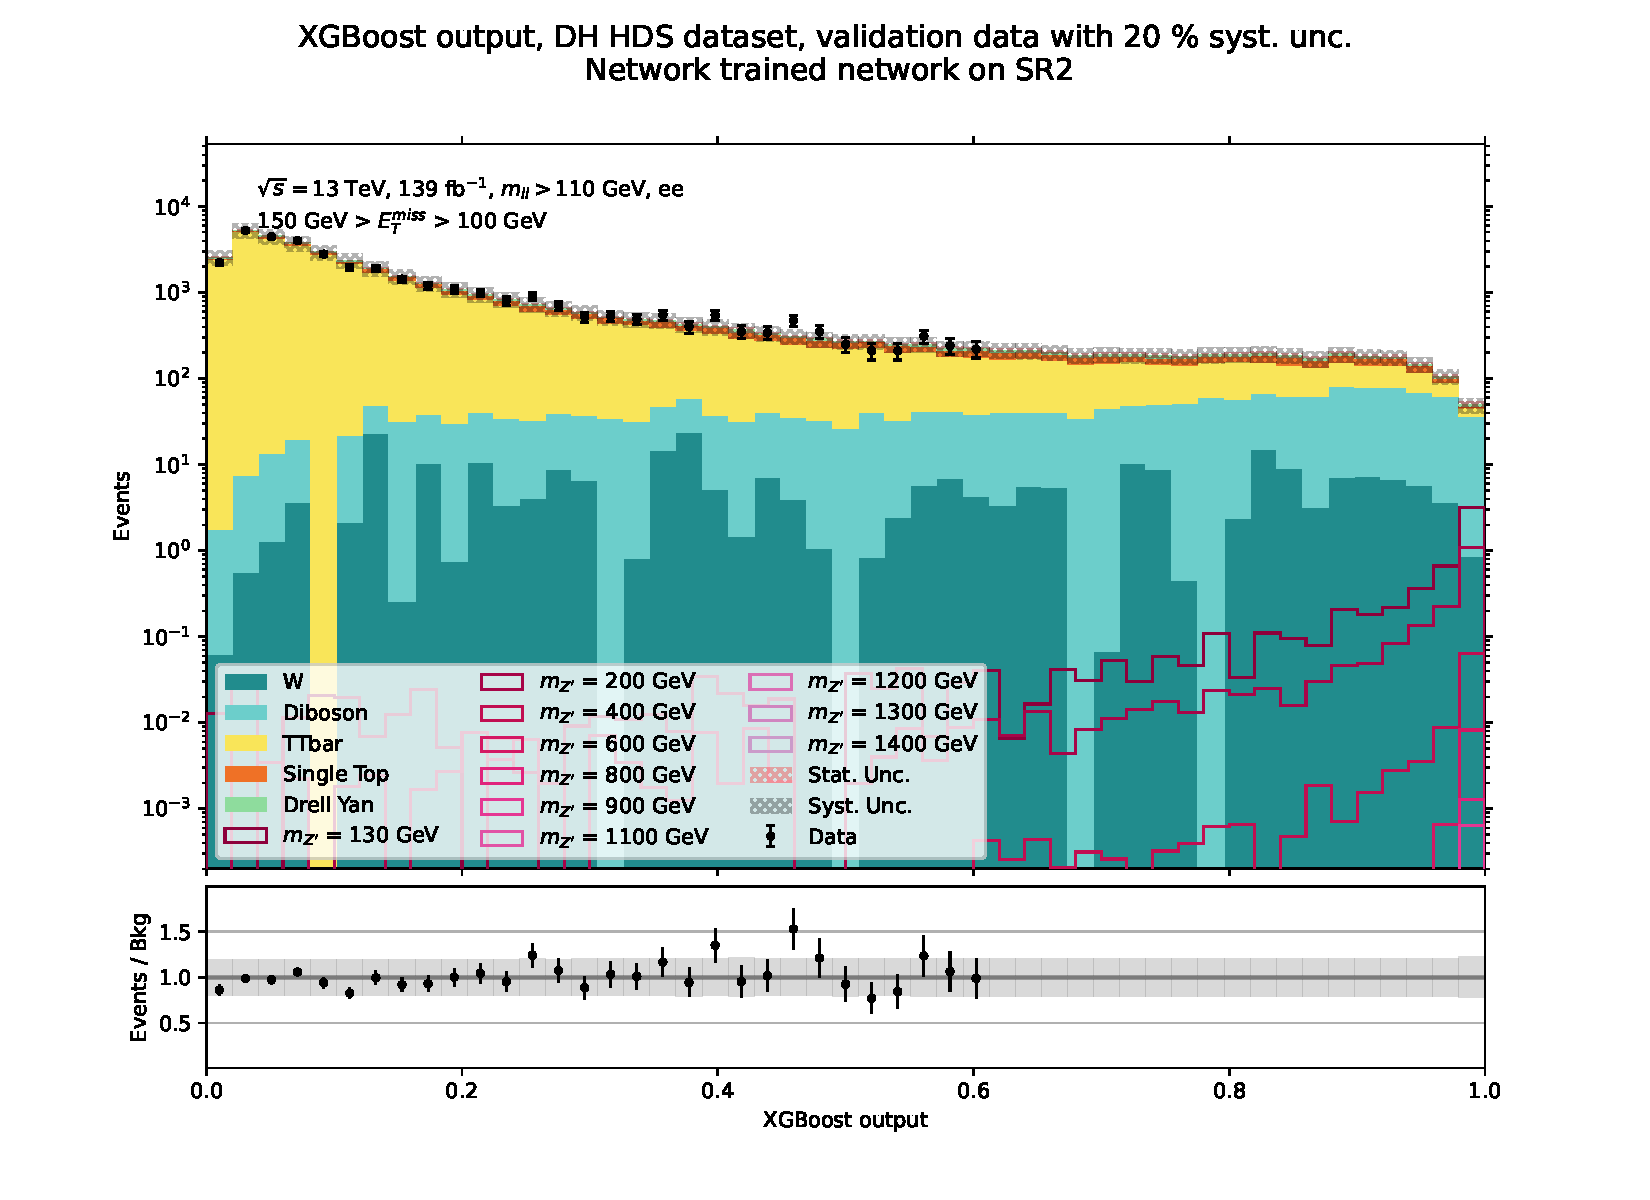
\includegraphics[width=1\textwidth]{XGBoost/Model_independent/100-150/DH_HDS/VAL_ee.pdf}
   \end{subfigure}
   \hfill
   \begin{subfigure}[b]{0.49\textwidth}
      \centering
      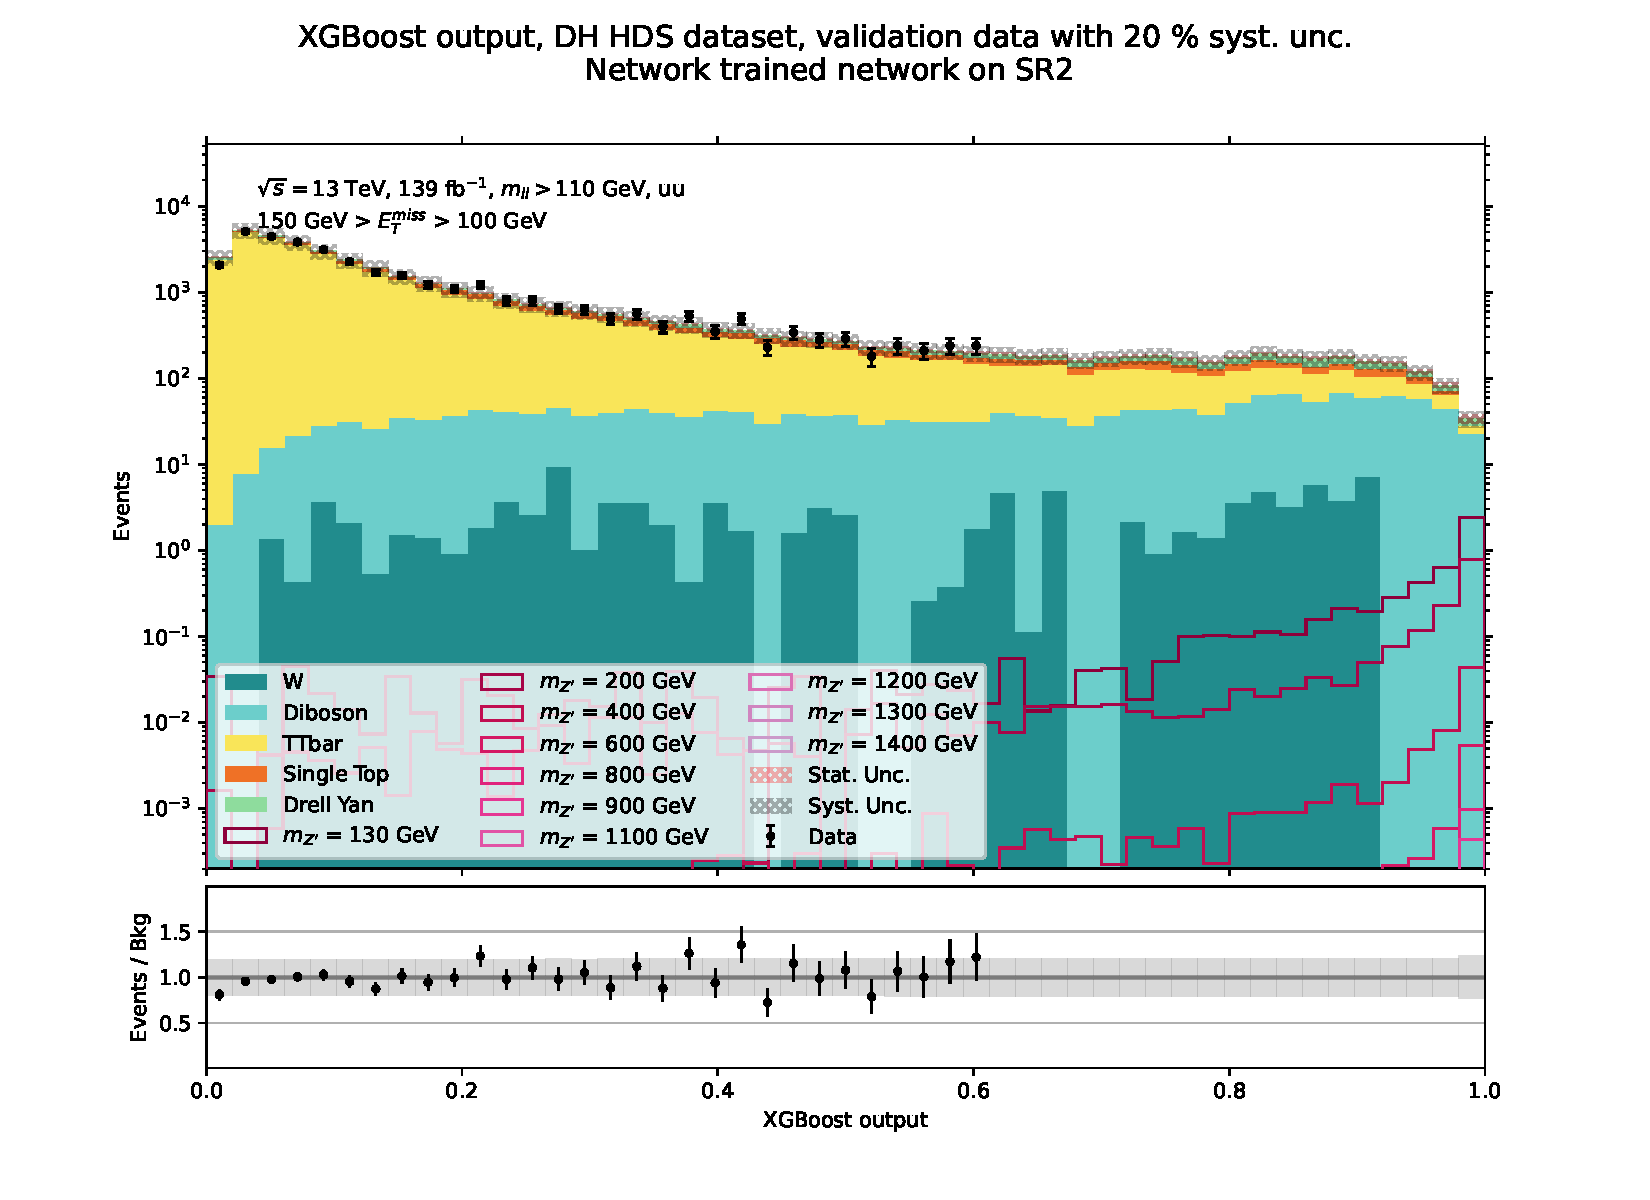
\includegraphics[width=1\textwidth]{XGBoost/Model_independent/100-150/DH_HDS/VAL_uu.pdf}
   \end{subfigure}
   \hfill
   \begin{subfigure}[b]{0.49\textwidth}
      \centering
      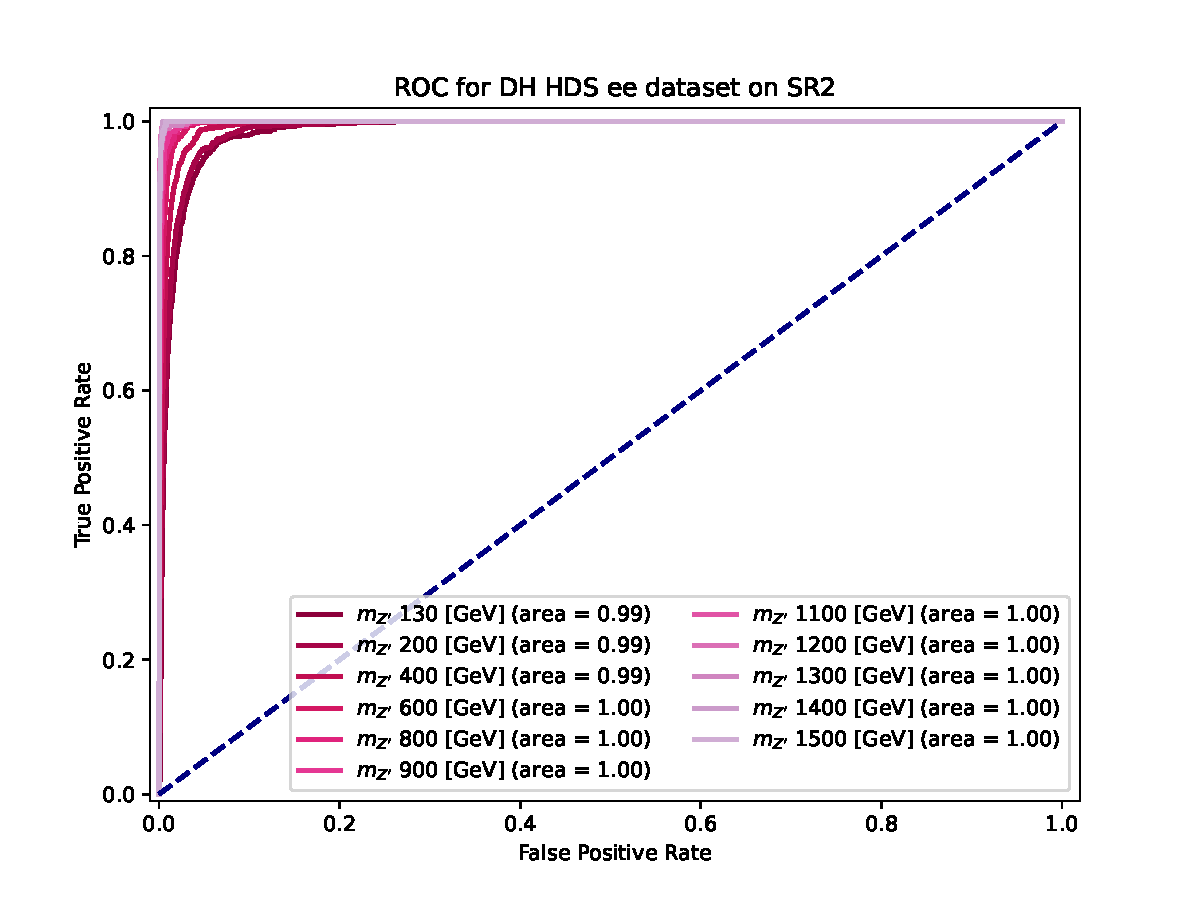
\includegraphics[width=1\textwidth]{XGBoost/Model_independent/100-150/DH_HDS/ROC_ee.pdf}
   \end{subfigure}
   \hfill
   \begin{subfigure}[b]{0.49\textwidth}
      \centering
      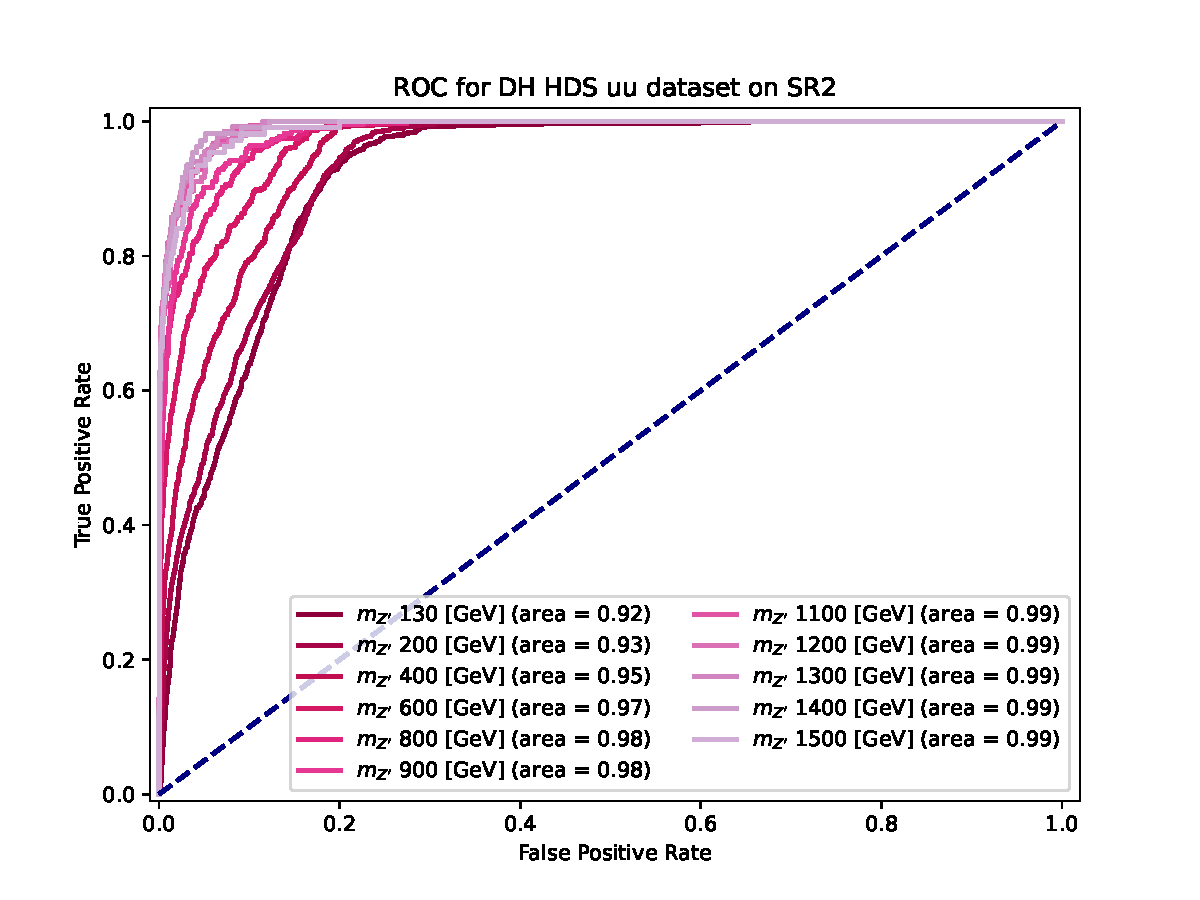
\includegraphics[width=1\textwidth]{XGBoost/Model_independent/100-150/DH_HDS/ROC_uu.pdf}
   \end{subfigure}
   \hfill
	\begin{subfigure}[b]{0.49\textwidth}
      \centering
      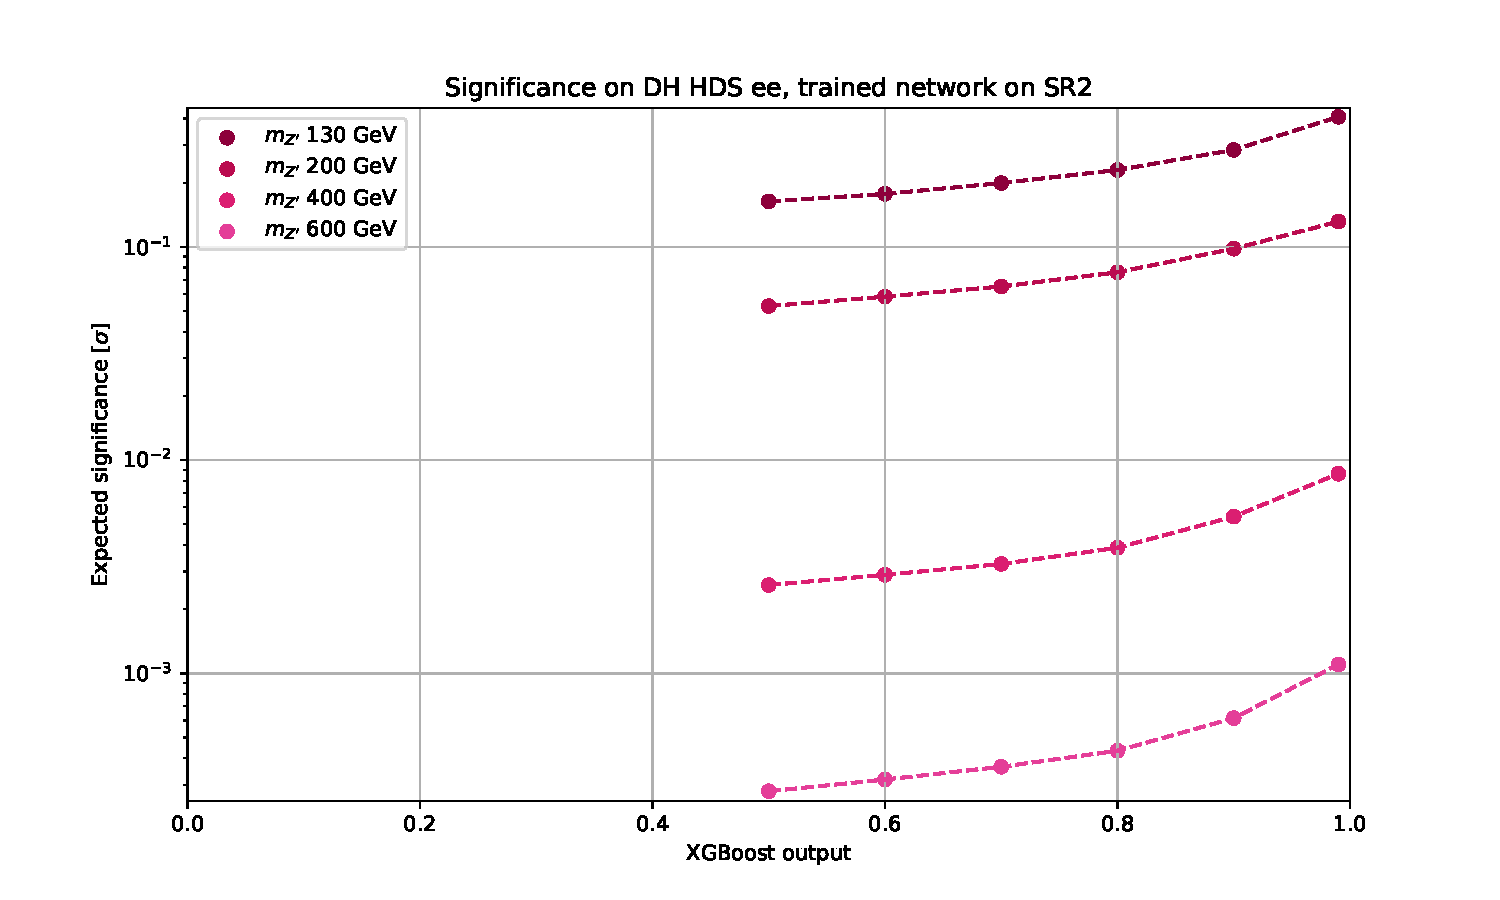
\includegraphics[width=1\textwidth]{XGBoost/Model_independent/100-150/DH_HDS/EXP_SIG_ee.pdf}
   \end{subfigure}
   \hfill
   \begin{subfigure}[b]{0.49\textwidth}
      \centering
      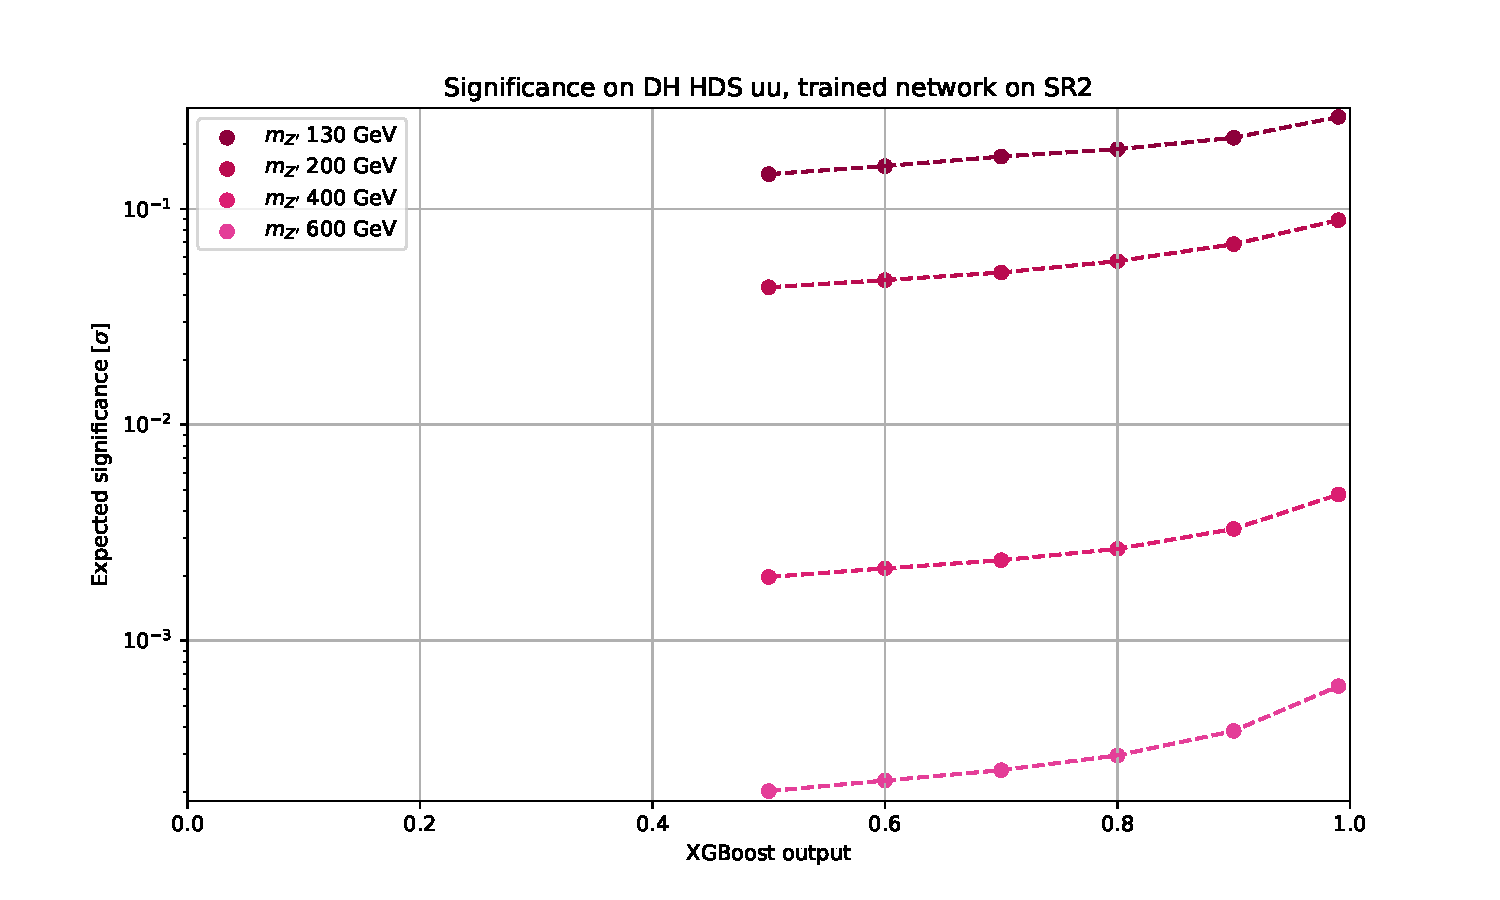
\includegraphics[width=1\textwidth]{XGBoost/Model_independent/100-150/DH_HDS/EXP_SIG_uu.pdf}
   \end{subfigure}
   \caption{XGBoost results for DH HDS model on $ee$ and $\mu\mu$ channel in SR2}\label{fig:DH_HDS_SR2}
\end{figure}
\begin{figure}[!ht]
	\centering
	\begin{subfigure}[b]{0.49\textwidth}
      \centering
      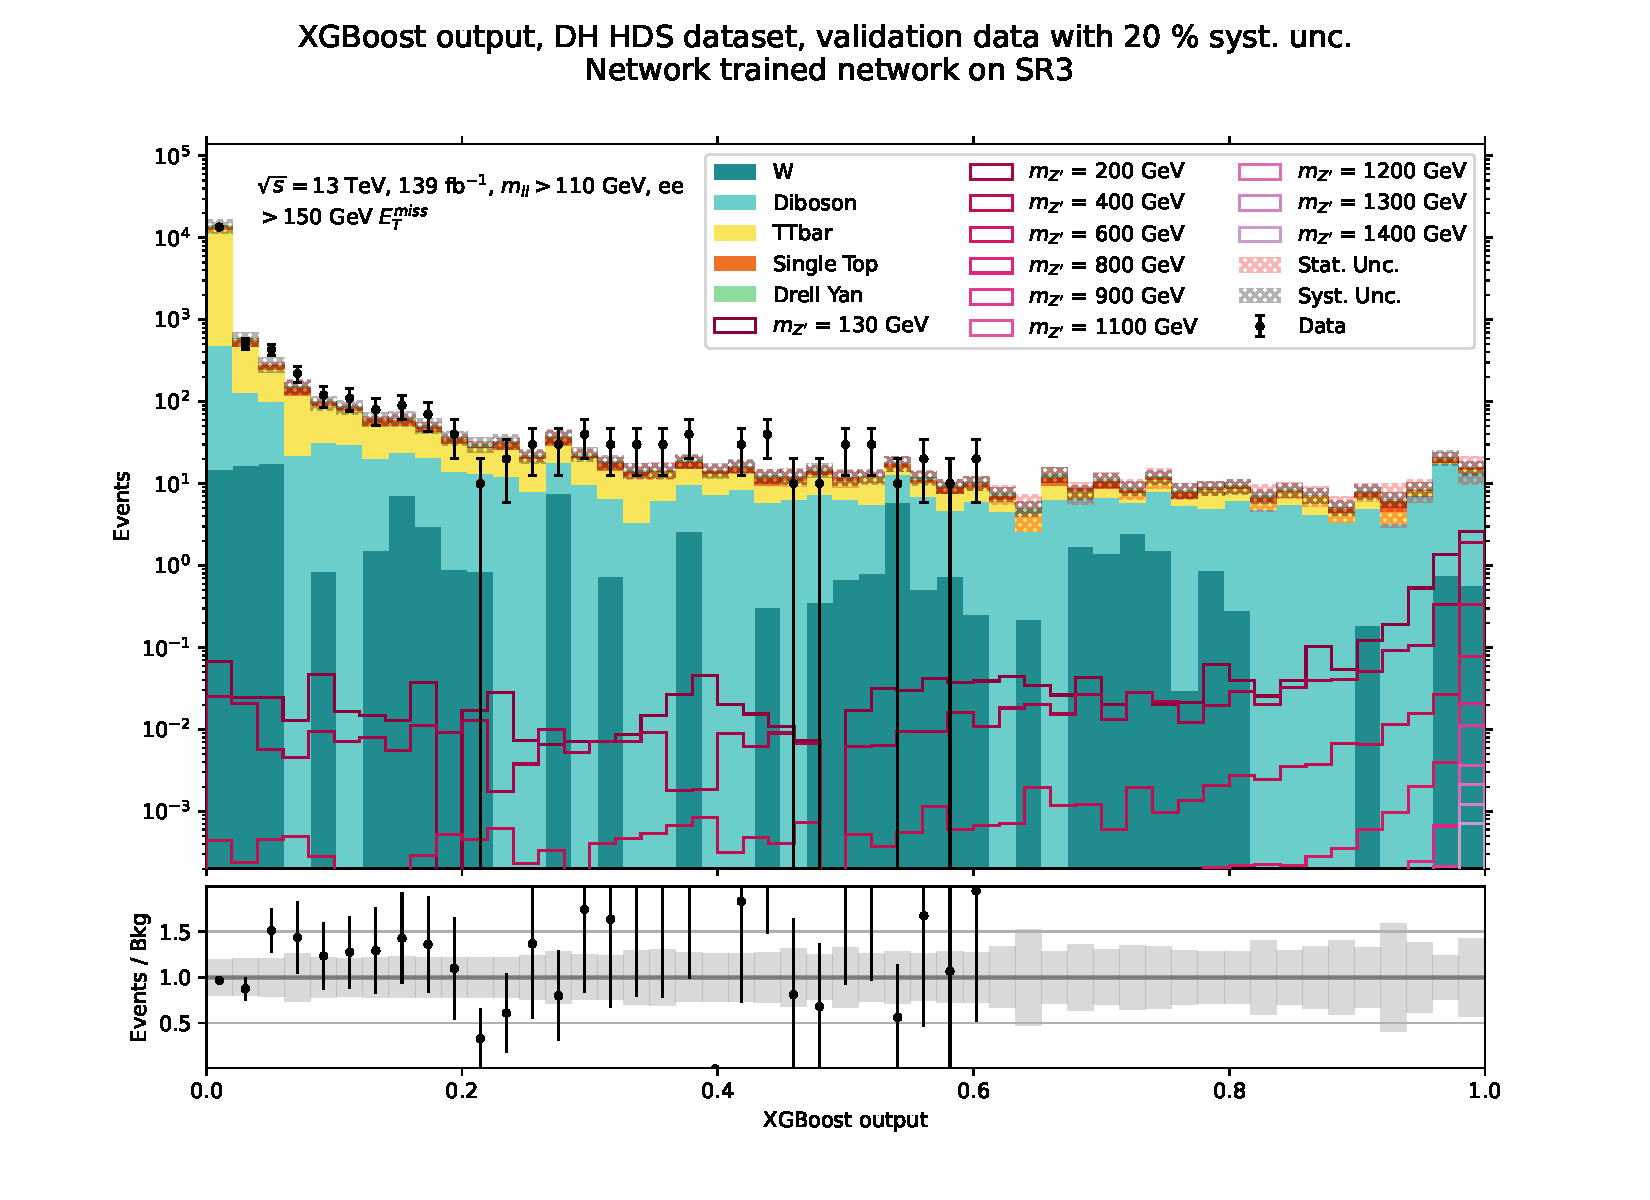
\includegraphics[width=1\textwidth]{XGBoost/Model_independent/150/DH_HDS/VAL_ee.pdf}
   \end{subfigure}
   \hfill
   \begin{subfigure}[b]{0.49\textwidth}
      \centering
      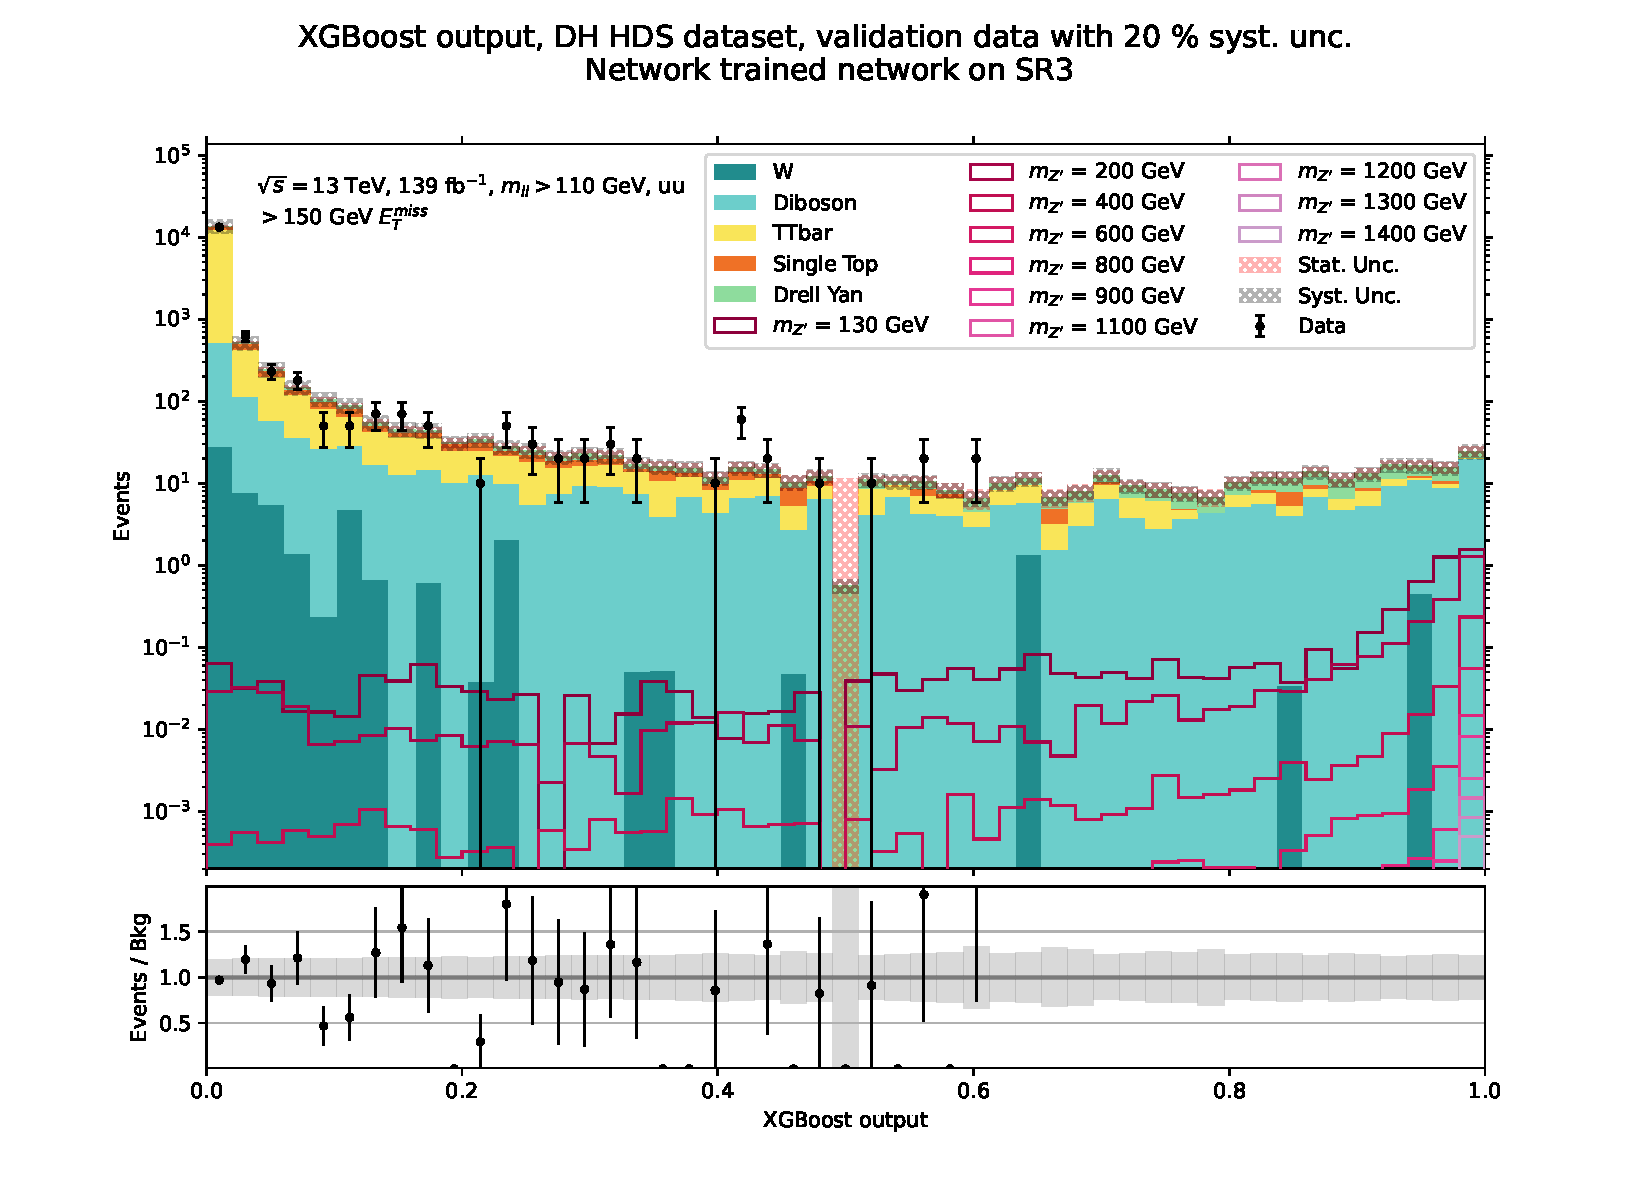
\includegraphics[width=1\textwidth]{XGBoost/Model_independent/150/DH_HDS/VAL_uu.pdf}
   \end{subfigure}
   \hfill
   \begin{subfigure}[b]{0.49\textwidth}
      \centering
      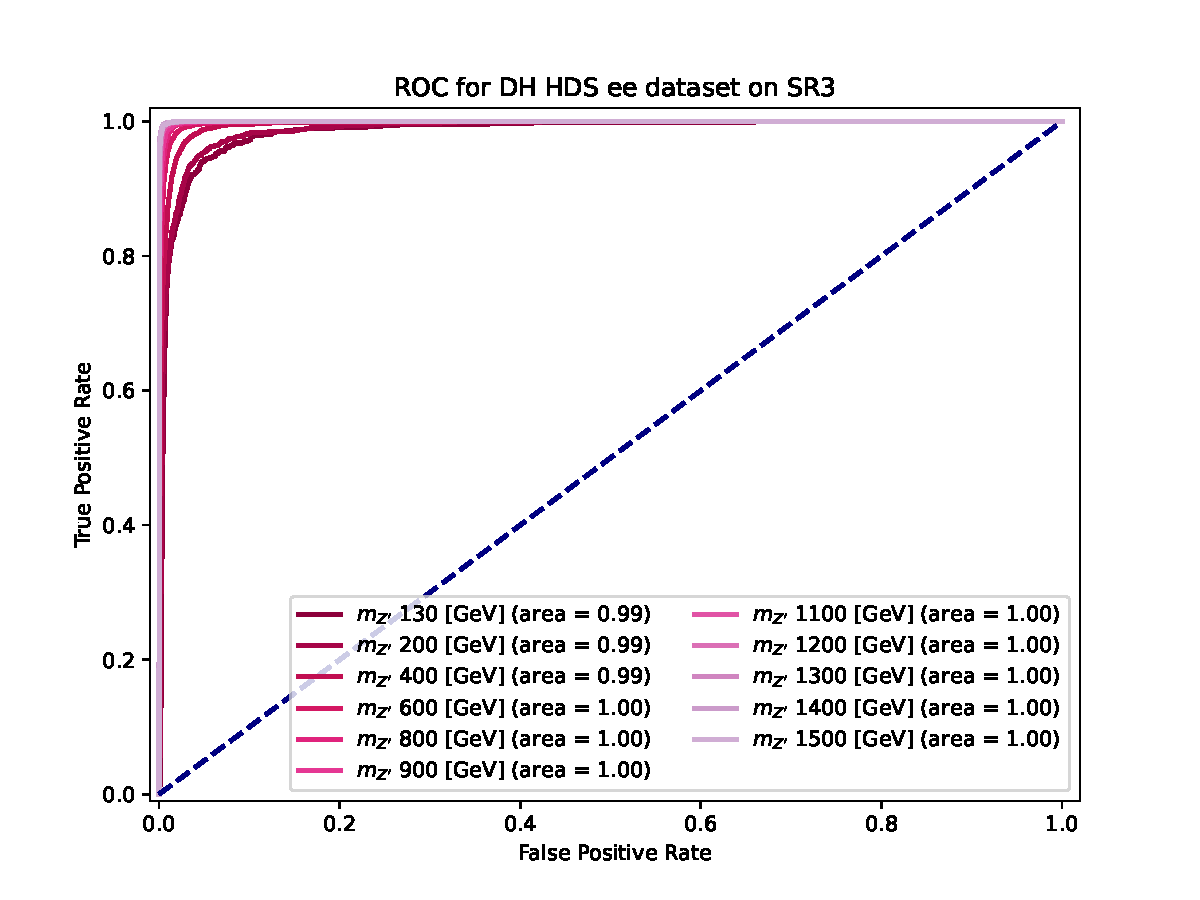
\includegraphics[width=1\textwidth]{XGBoost/Model_independent/150/DH_HDS/ROC_ee.pdf}
   \end{subfigure}
   \hfill
   \begin{subfigure}[b]{0.49\textwidth}
      \centering
      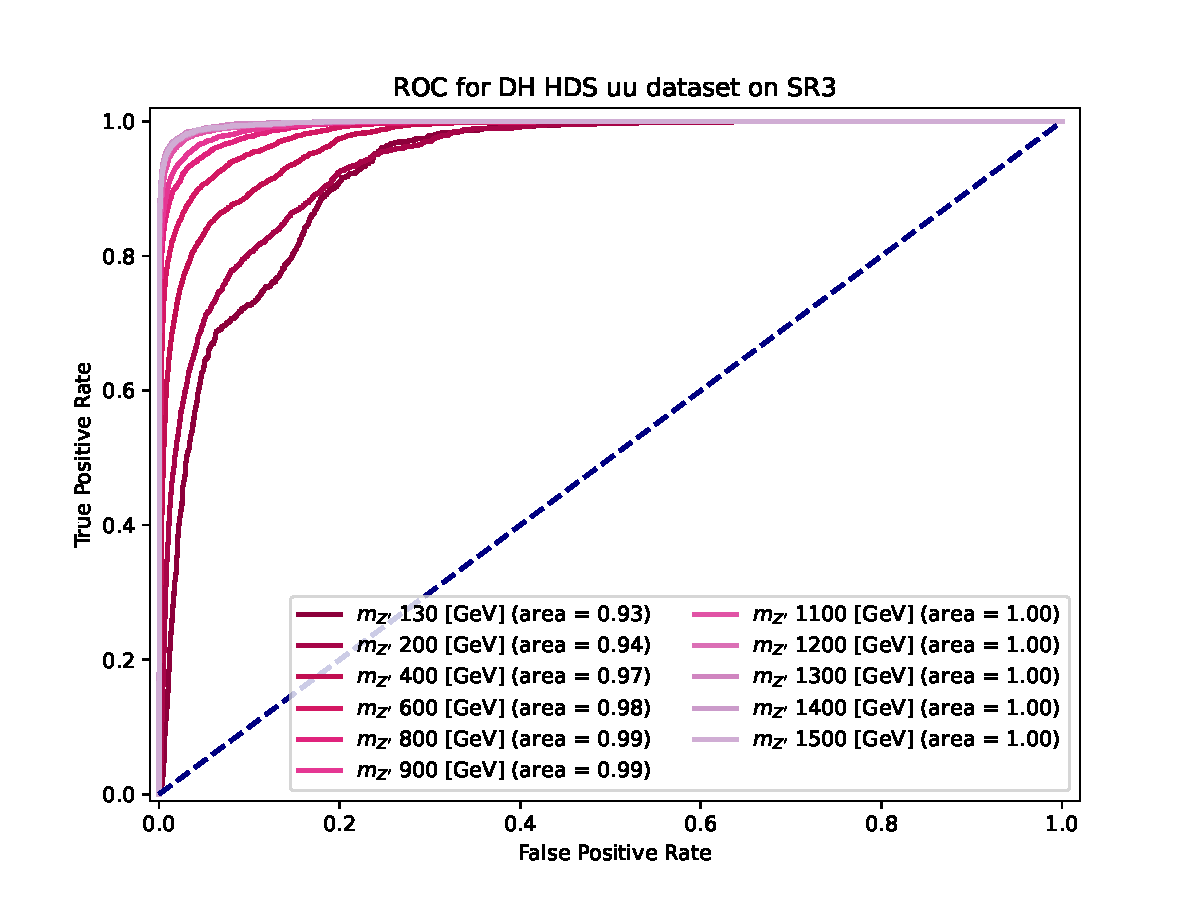
\includegraphics[width=1\textwidth]{XGBoost/Model_independent/150/DH_HDS/ROC_uu.pdf}
   \end{subfigure}
   \hfill
	\begin{subfigure}[b]{0.49\textwidth}
      \centering
      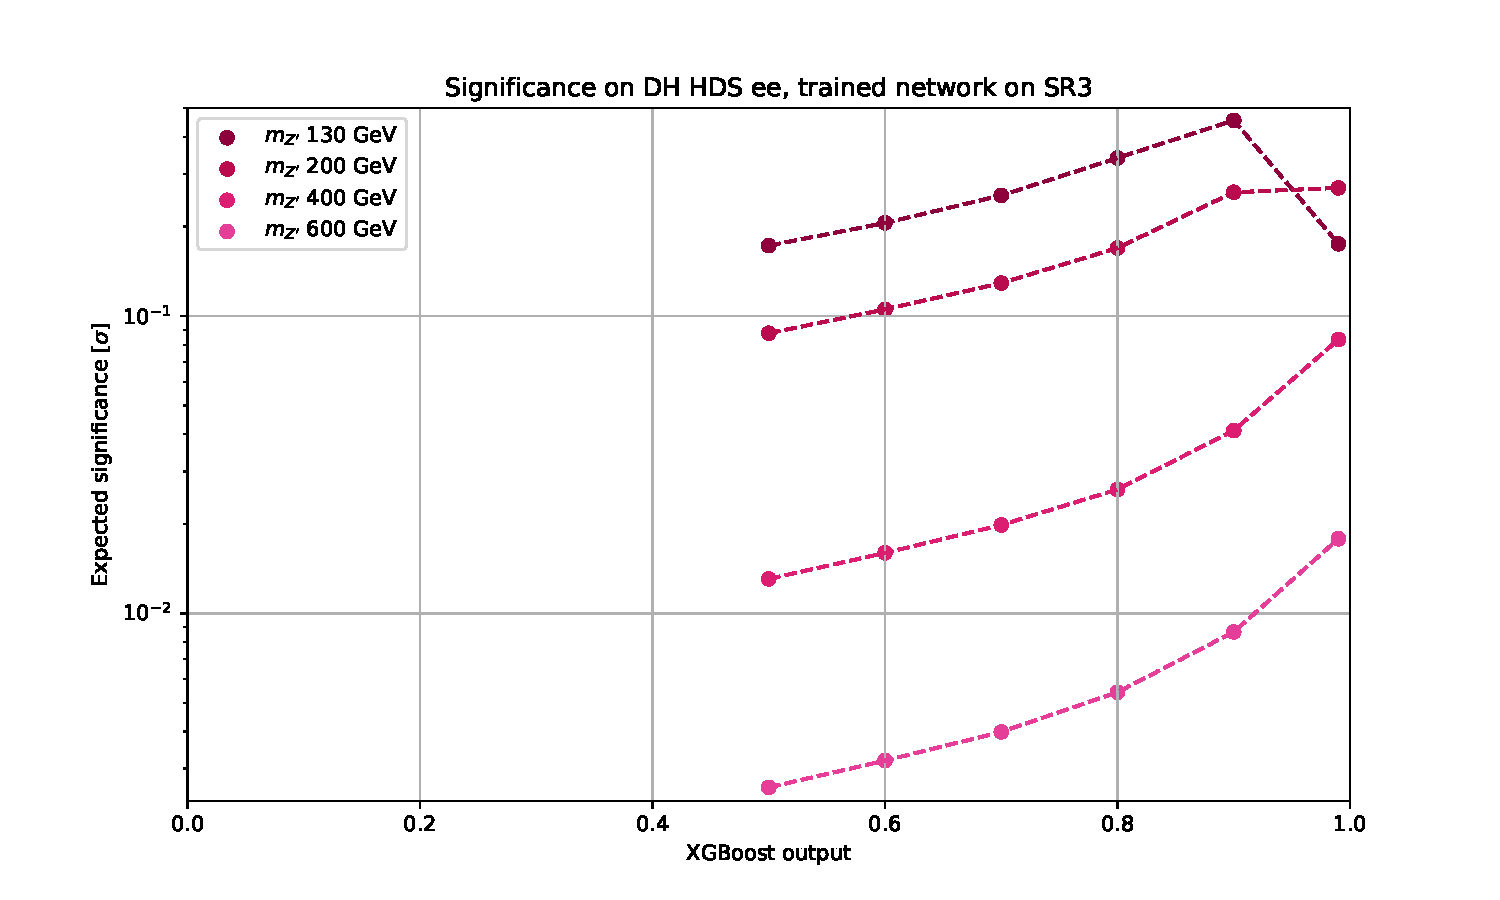
\includegraphics[width=1\textwidth]{XGBoost/Model_independent/150/DH_HDS/EXP_SIG_ee.pdf}
   \end{subfigure}
   \hfill
   \begin{subfigure}[b]{0.49\textwidth}
      \centering
      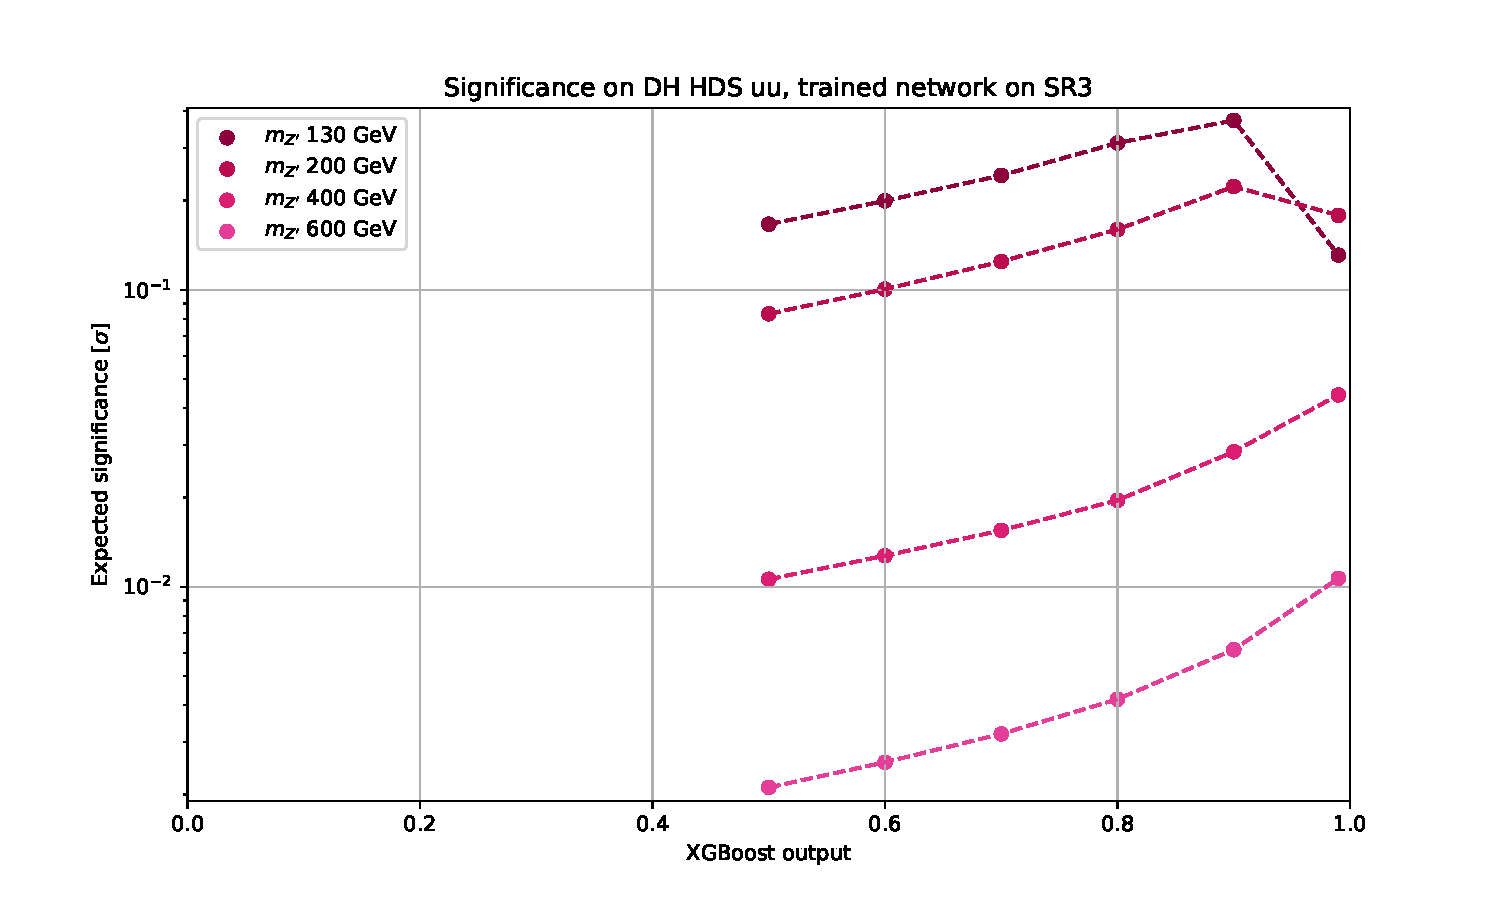
\includegraphics[width=1\textwidth]{XGBoost/Model_independent/150/DH_HDS/EXP_SIG_uu.pdf}
   \end{subfigure}
   \caption{XGBoost results for DH HDS model on $ee$ and $\mu\mu$ channel in SR3}\label{fig:DH_HDS_SR3}
\end{figure}
\\Using again the last bin of the validation set to make a cut on the dataset to make limits, we get the values seen is Table \ref{tab:stat_vals_DH_HDS_SR1}, \ref{tab:stat_vals_DH_HDS_SR2} and \ref{tab:stat_vals_DH_HDS_SR3} for 
SR1, SR2 and SR3 respectively. Using these to compute limits for the electron and muon channel for every SR using the method explained in Chapter \ref{sec:stat_anal} we get the exclusion plots shown in Figure \ref{fig:DH_HDS_me_SRS}.\\
\begin{figure}[!ht]
	\centering
	\begin{subfigure}[b]{0.49\textwidth}
      \centering
      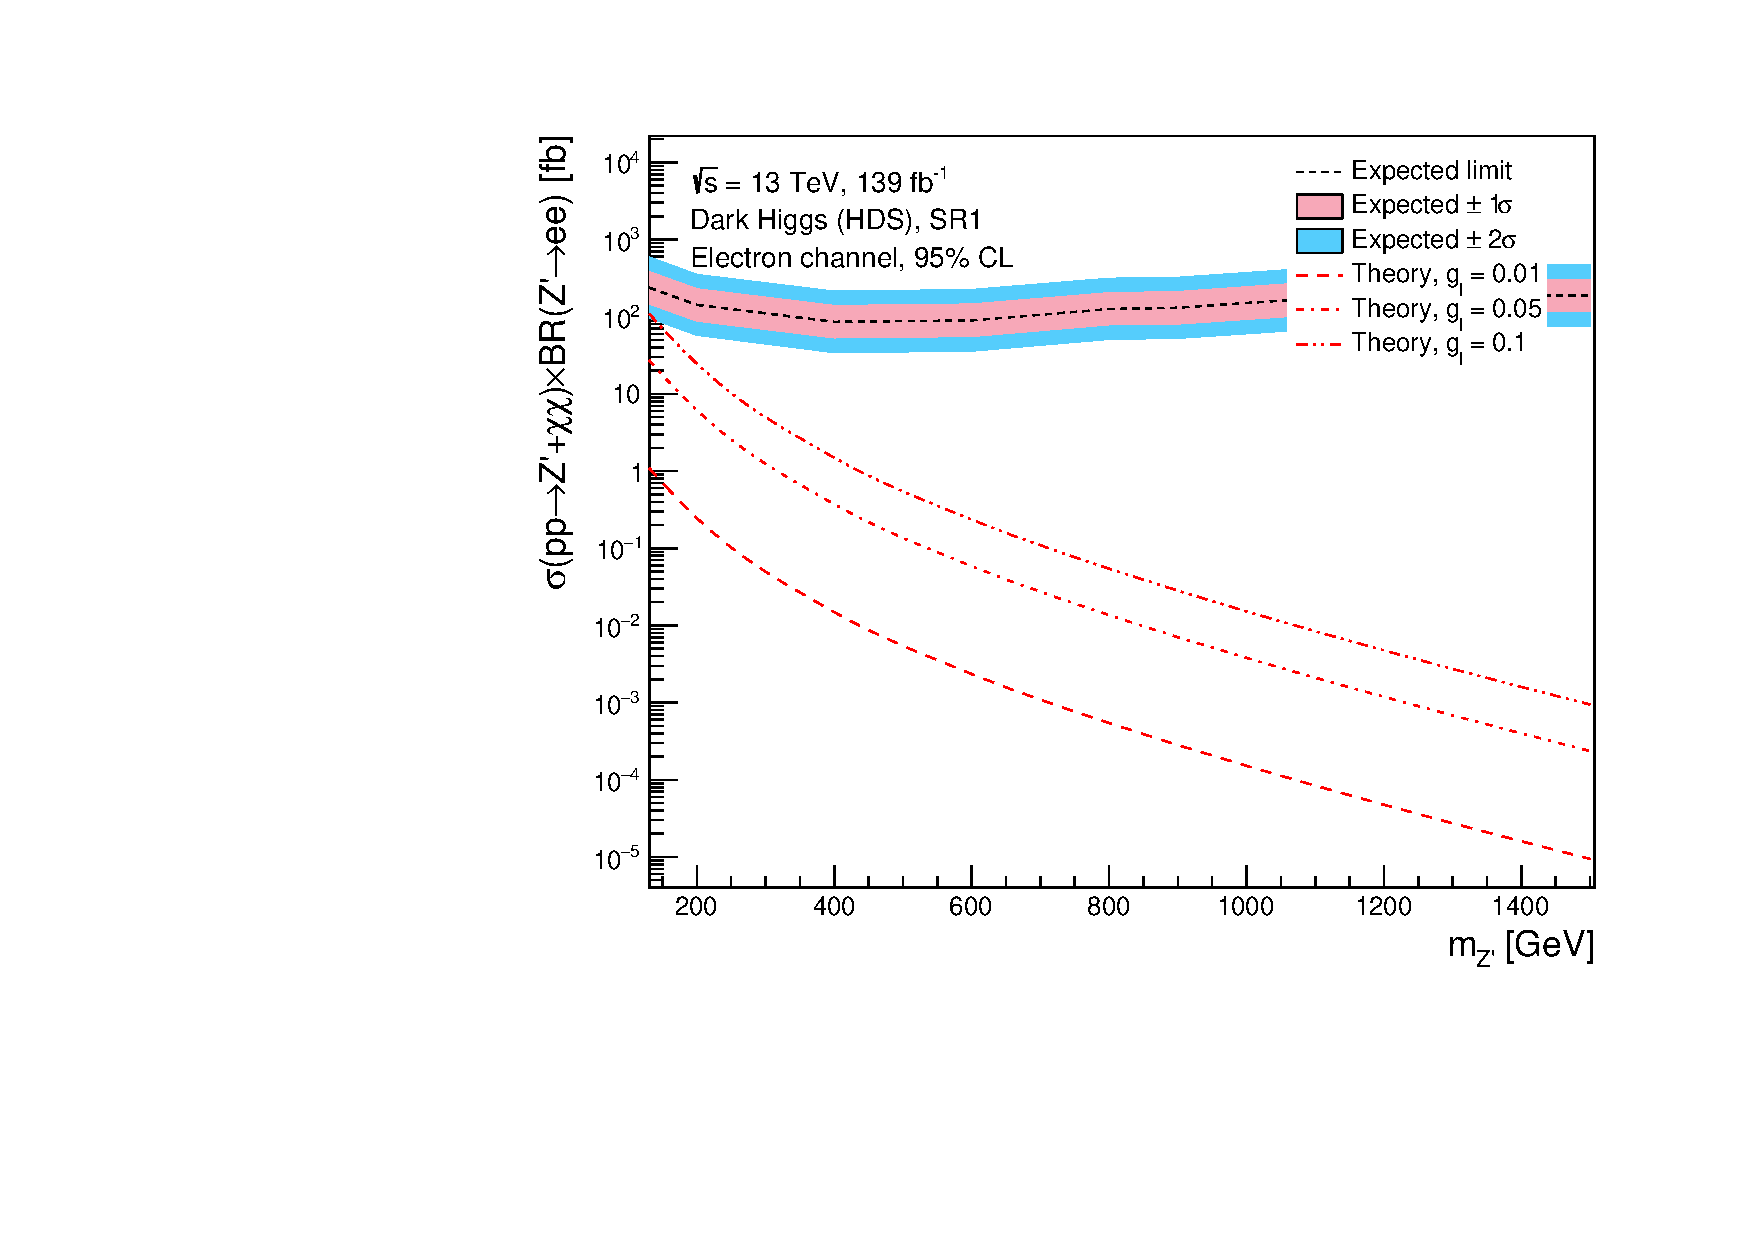
\includegraphics[width=1\textwidth]{Limits/Model_independent/50-100/DH_HDS/mass_exclusion_ee.pdf}
   \end{subfigure}
   \hfill
   \begin{subfigure}[b]{0.49\textwidth}
      \centering
      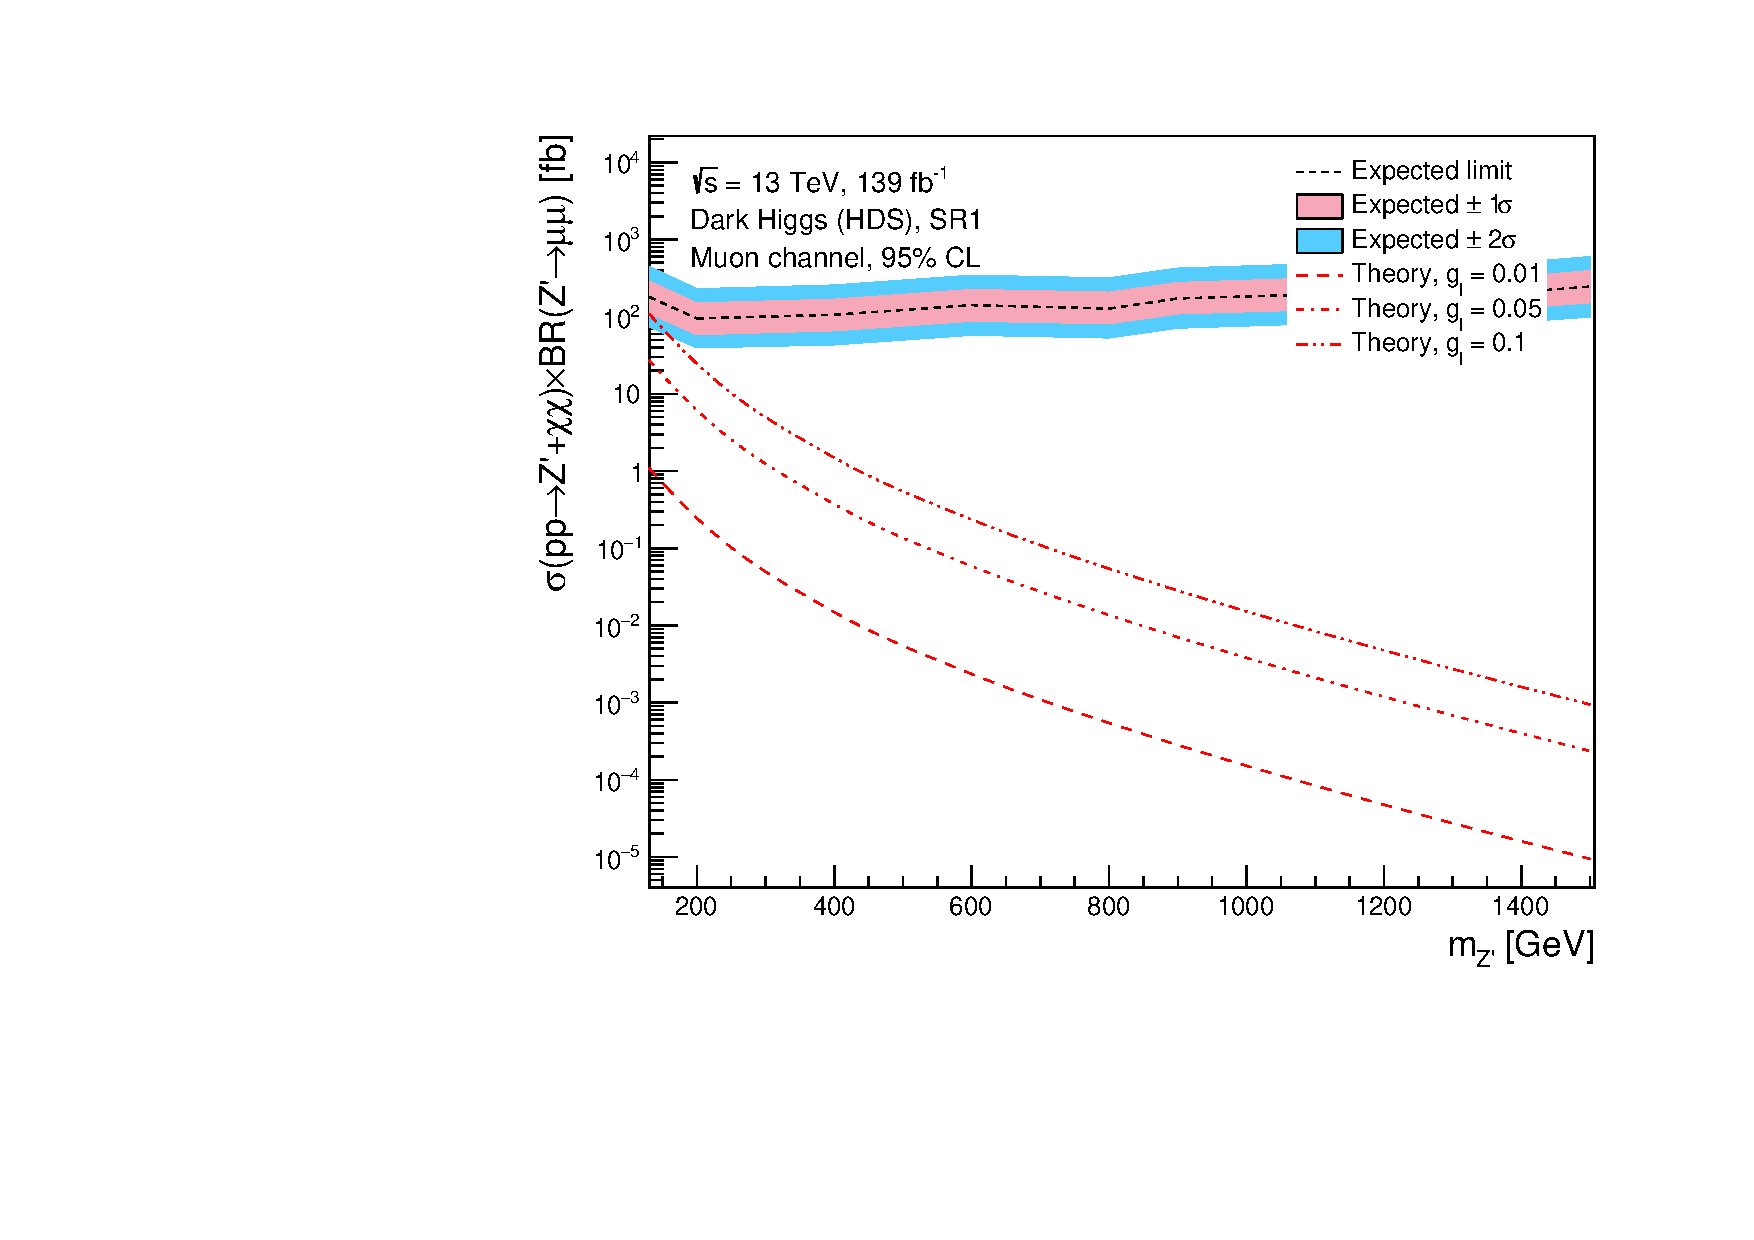
\includegraphics[width=1\textwidth]{Limits/Model_independent/50-100/DH_HDS/mass_exclusion_uu.pdf}
   \end{subfigure}
   \hfill
   \begin{subfigure}[b]{0.49\textwidth}
      \centering
      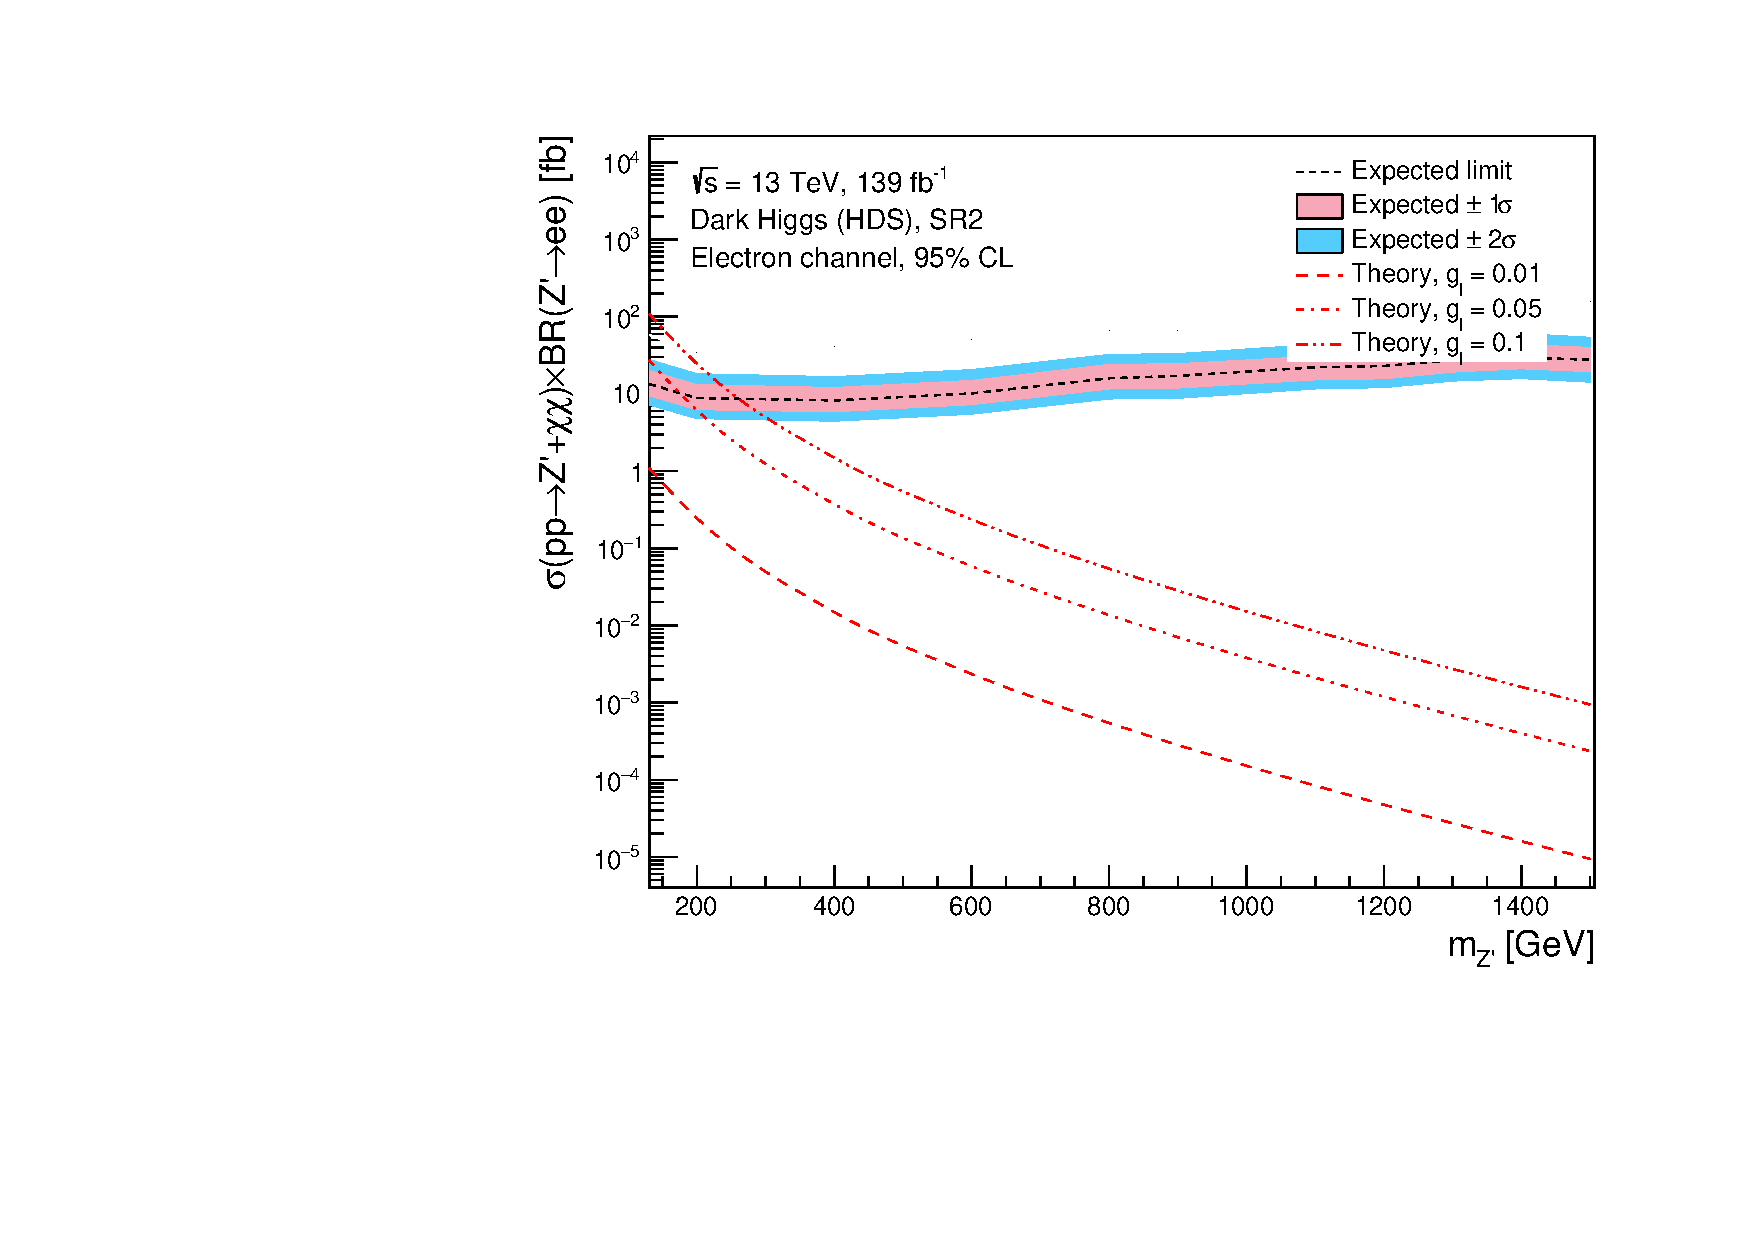
\includegraphics[width=1\textwidth]{Limits/Model_independent/100-150/DH_HDS/mass_exclusion_ee.pdf}
   \end{subfigure}
   \hfill
   \begin{subfigure}[b]{0.49\textwidth}
      \centering
      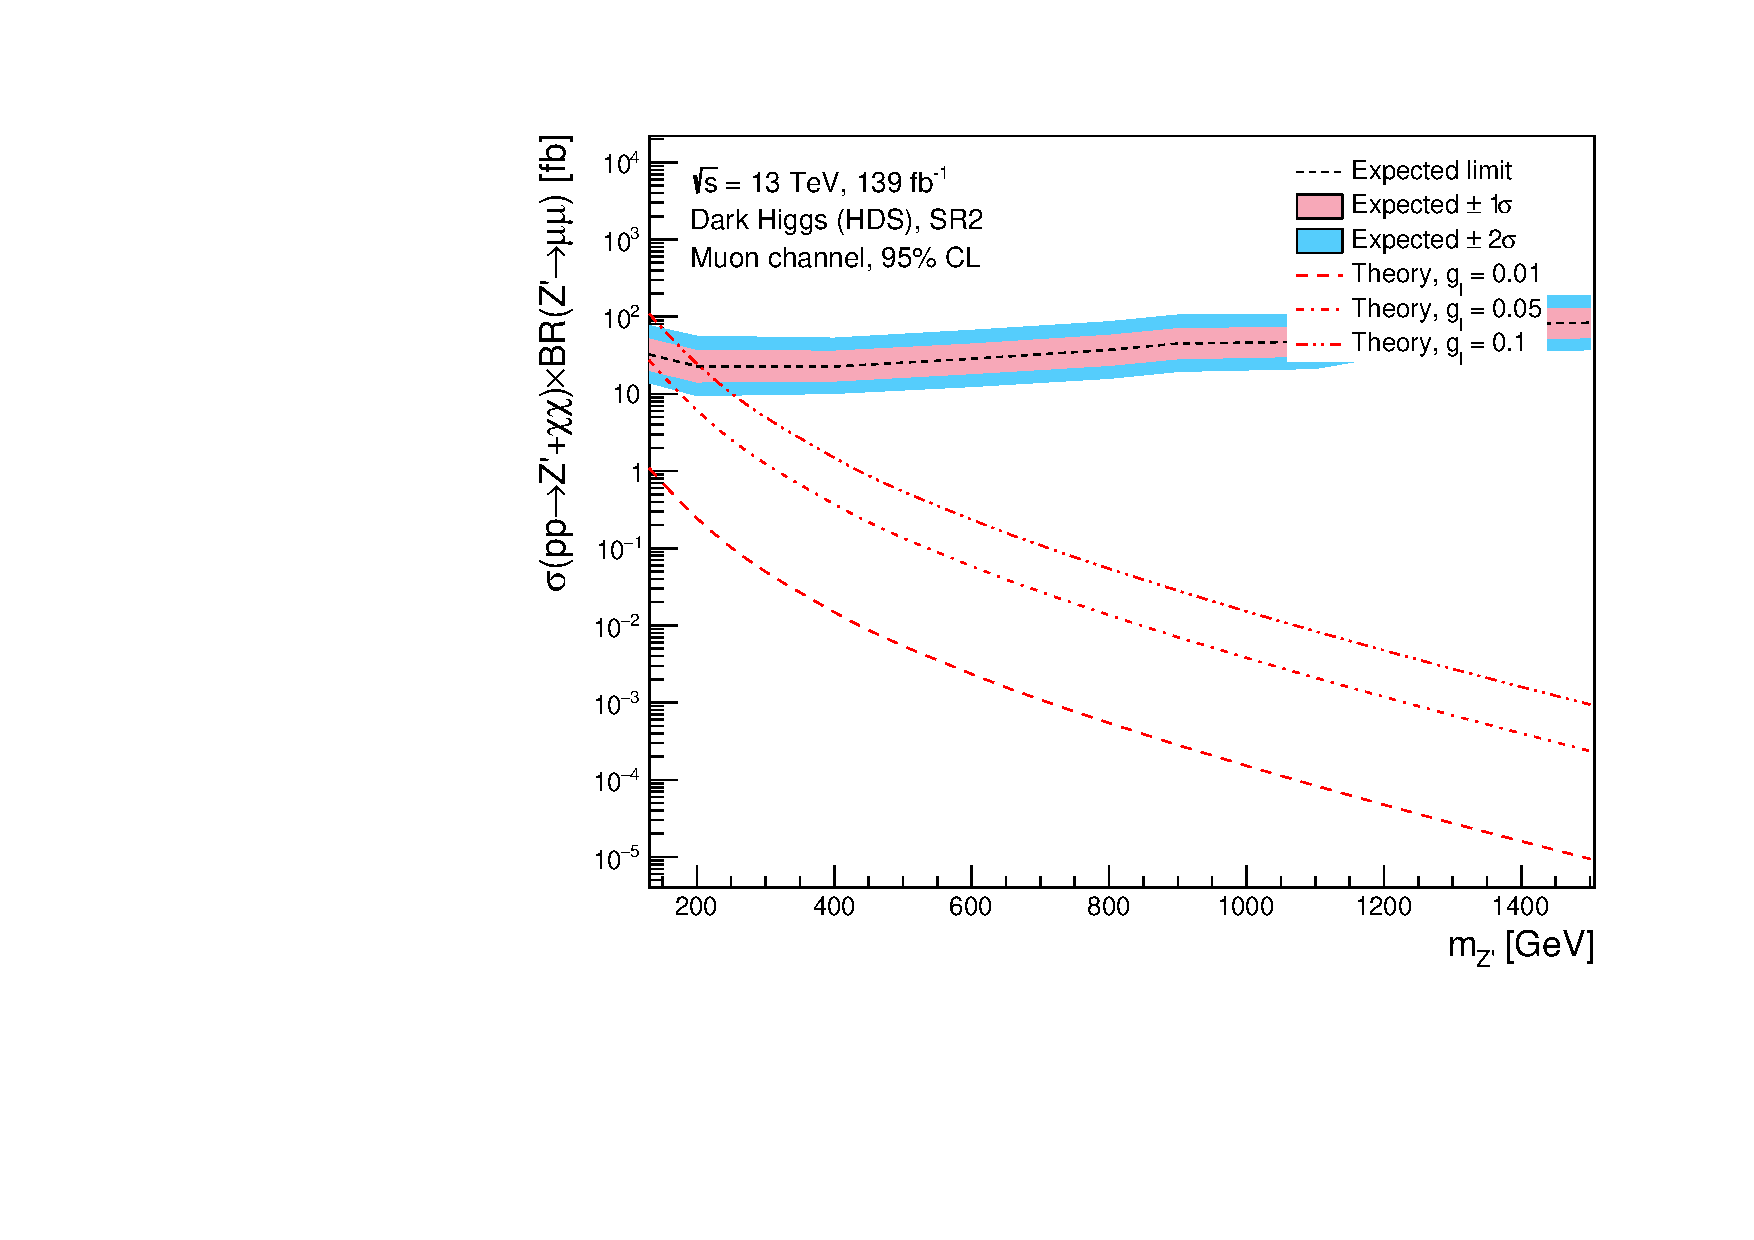
\includegraphics[width=1\textwidth]{Limits/Model_independent/100-150/DH_HDS/mass_exclusion_uu.pdf}
   \end{subfigure}
   \hfill
	\begin{subfigure}[b]{0.49\textwidth}
      \centering
      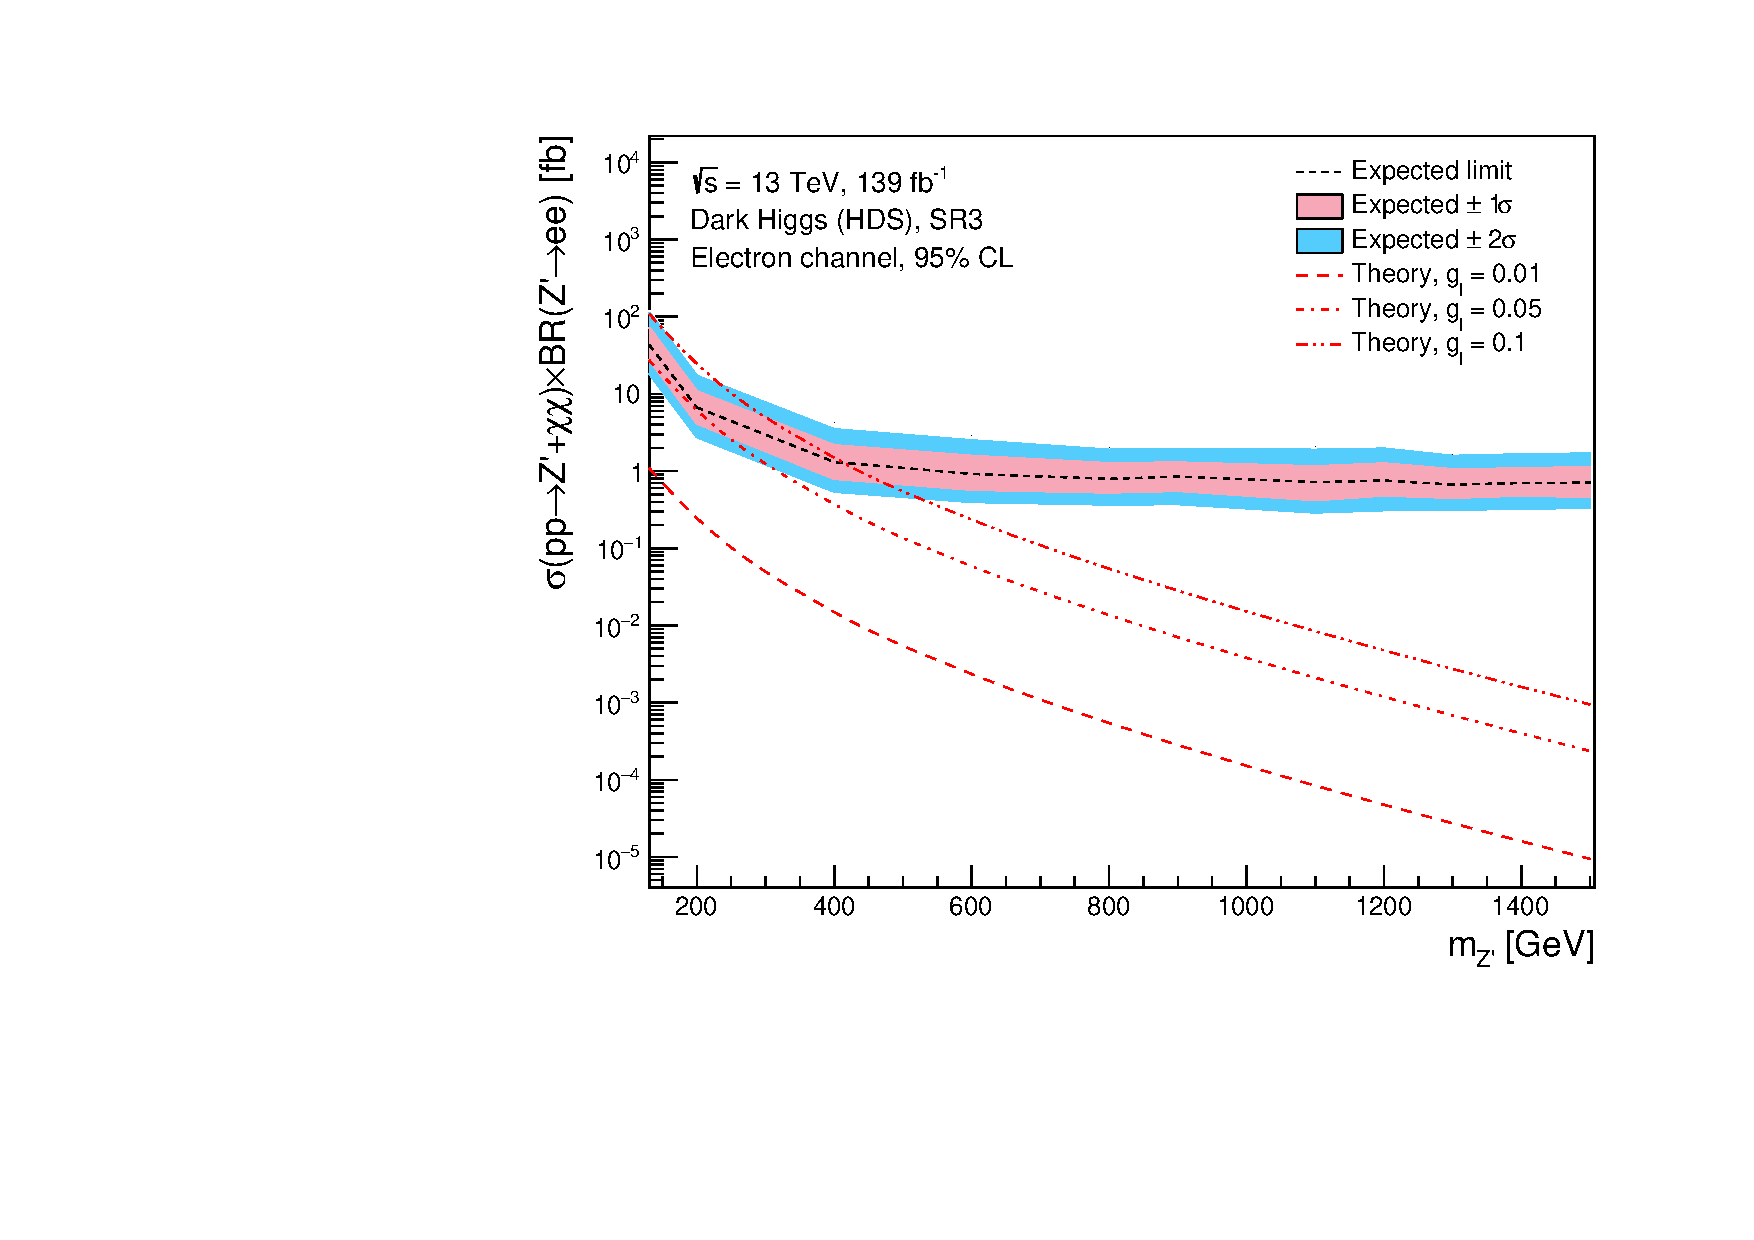
\includegraphics[width=1\textwidth]{Limits/Model_independent/150/DH_HDS/mass_exclusion_ee.pdf}
   \end{subfigure}
   \hfill
   \begin{subfigure}[b]{0.49\textwidth}
      \centering
      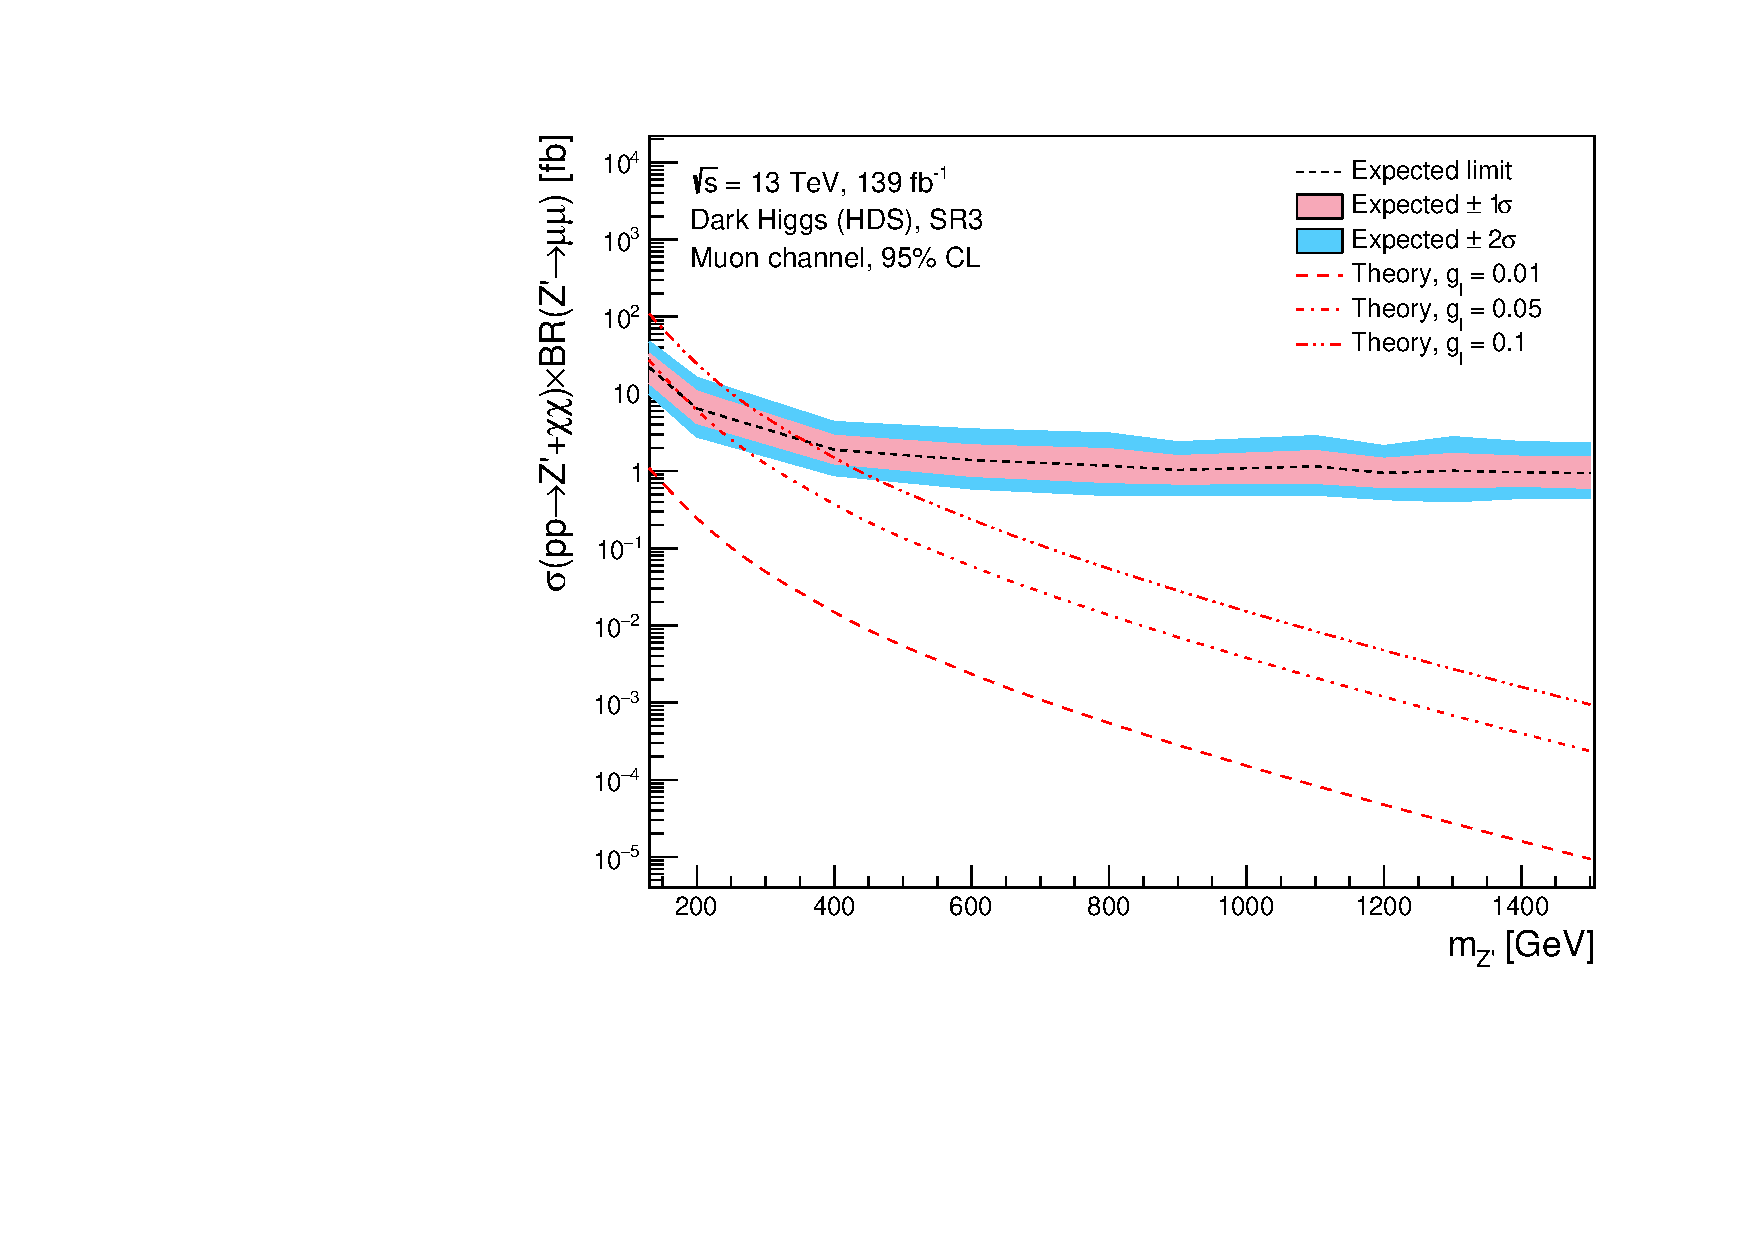
\includegraphics[width=1\textwidth]{Limits/Model_independent/150/DH_HDS/mass_exclusion_uu.pdf}
   \end{subfigure}
   \caption{Mass exclusion limits results for DH HDS model on $ee$ and $\mu\mu$ channel in all SRs}\label{fig:DH_HDS_me_SRS}
\end{figure} 
\\We can furthermore statistically combine the results for each SR such that we get the exclusion in Figure \ref{fig:DH_HDS_me_comb}. 
\begin{figure}[!ht]
	\centering
	\begin{subfigure}[b]{0.49\textwidth}
      \centering
      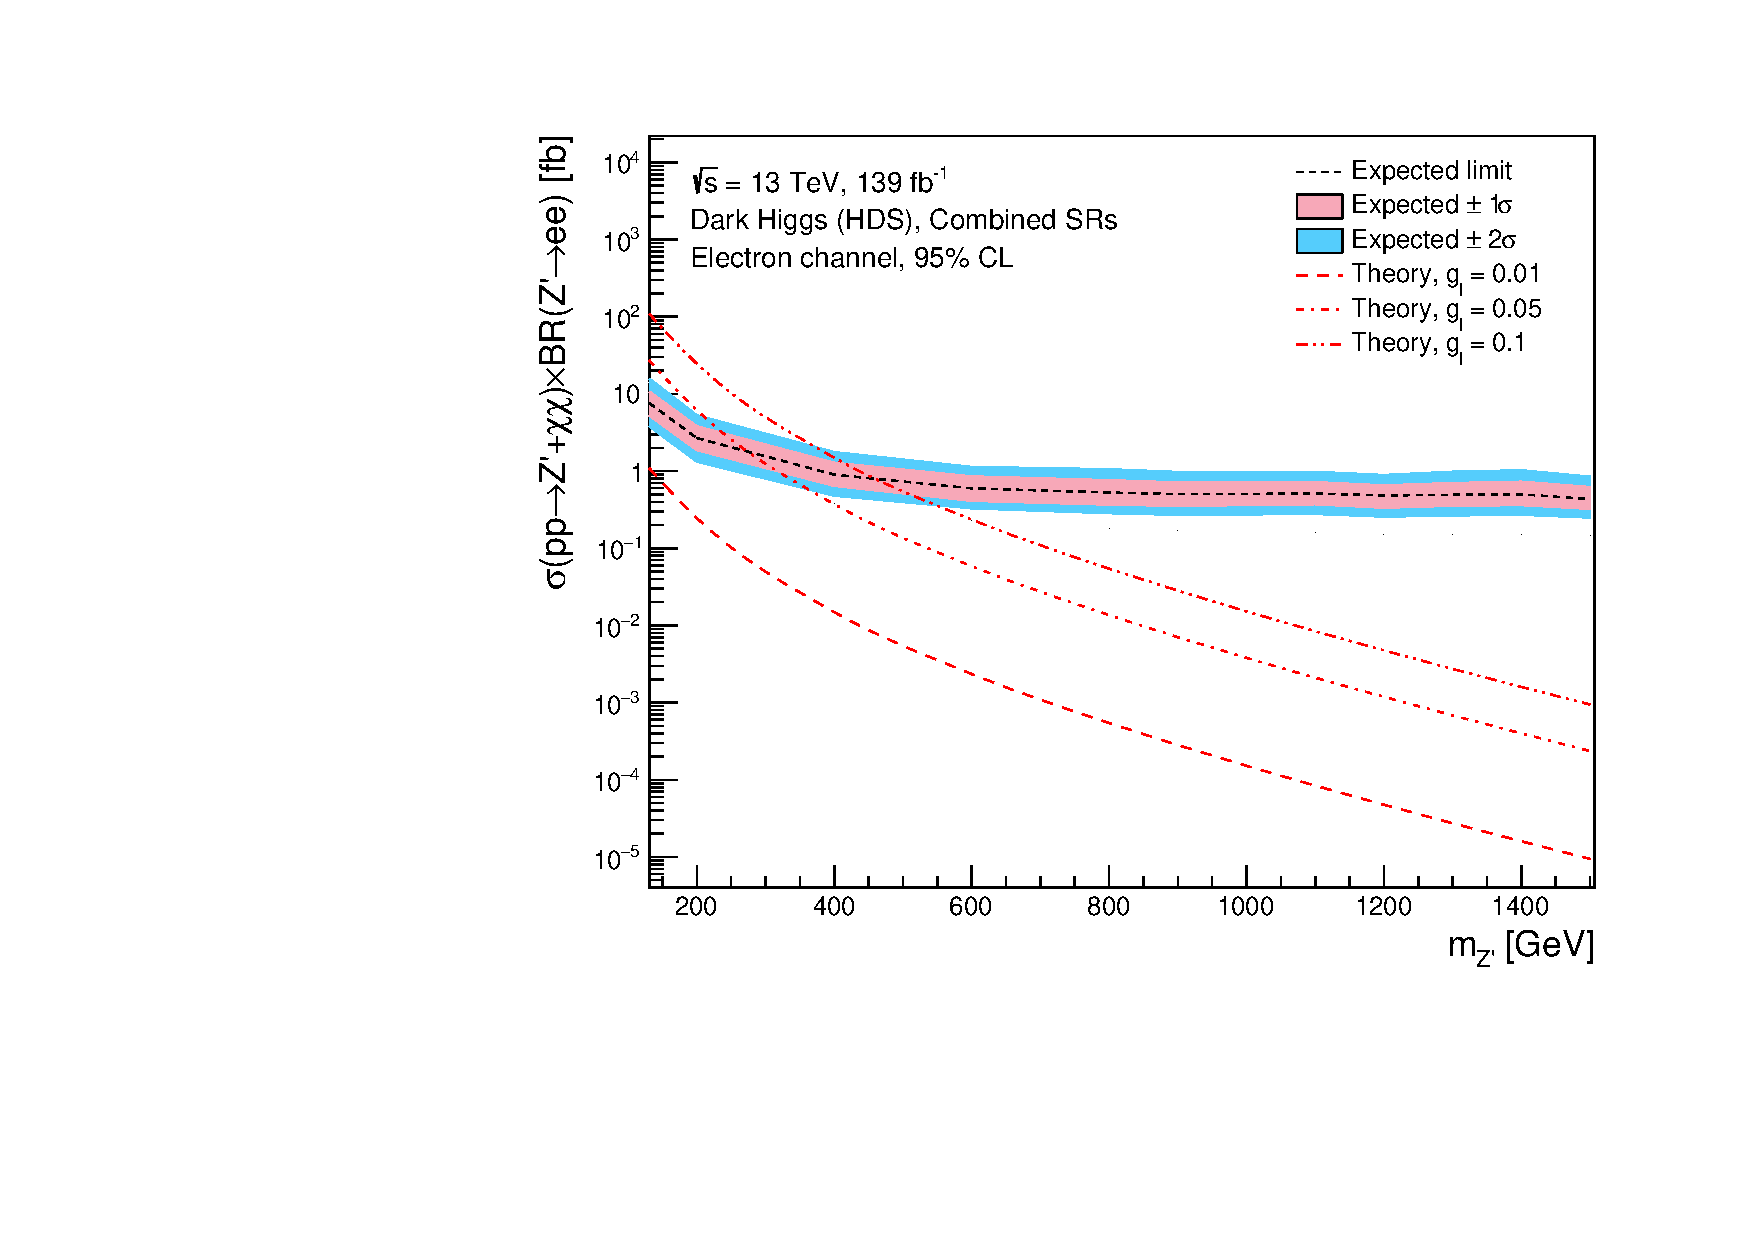
\includegraphics[width=1\textwidth]{Limits/Model_independent/DH_HDS/mass_exclusion_ee.pdf}
   \end{subfigure}
   \hfill
   \begin{subfigure}[b]{0.49\textwidth}
      \centering
      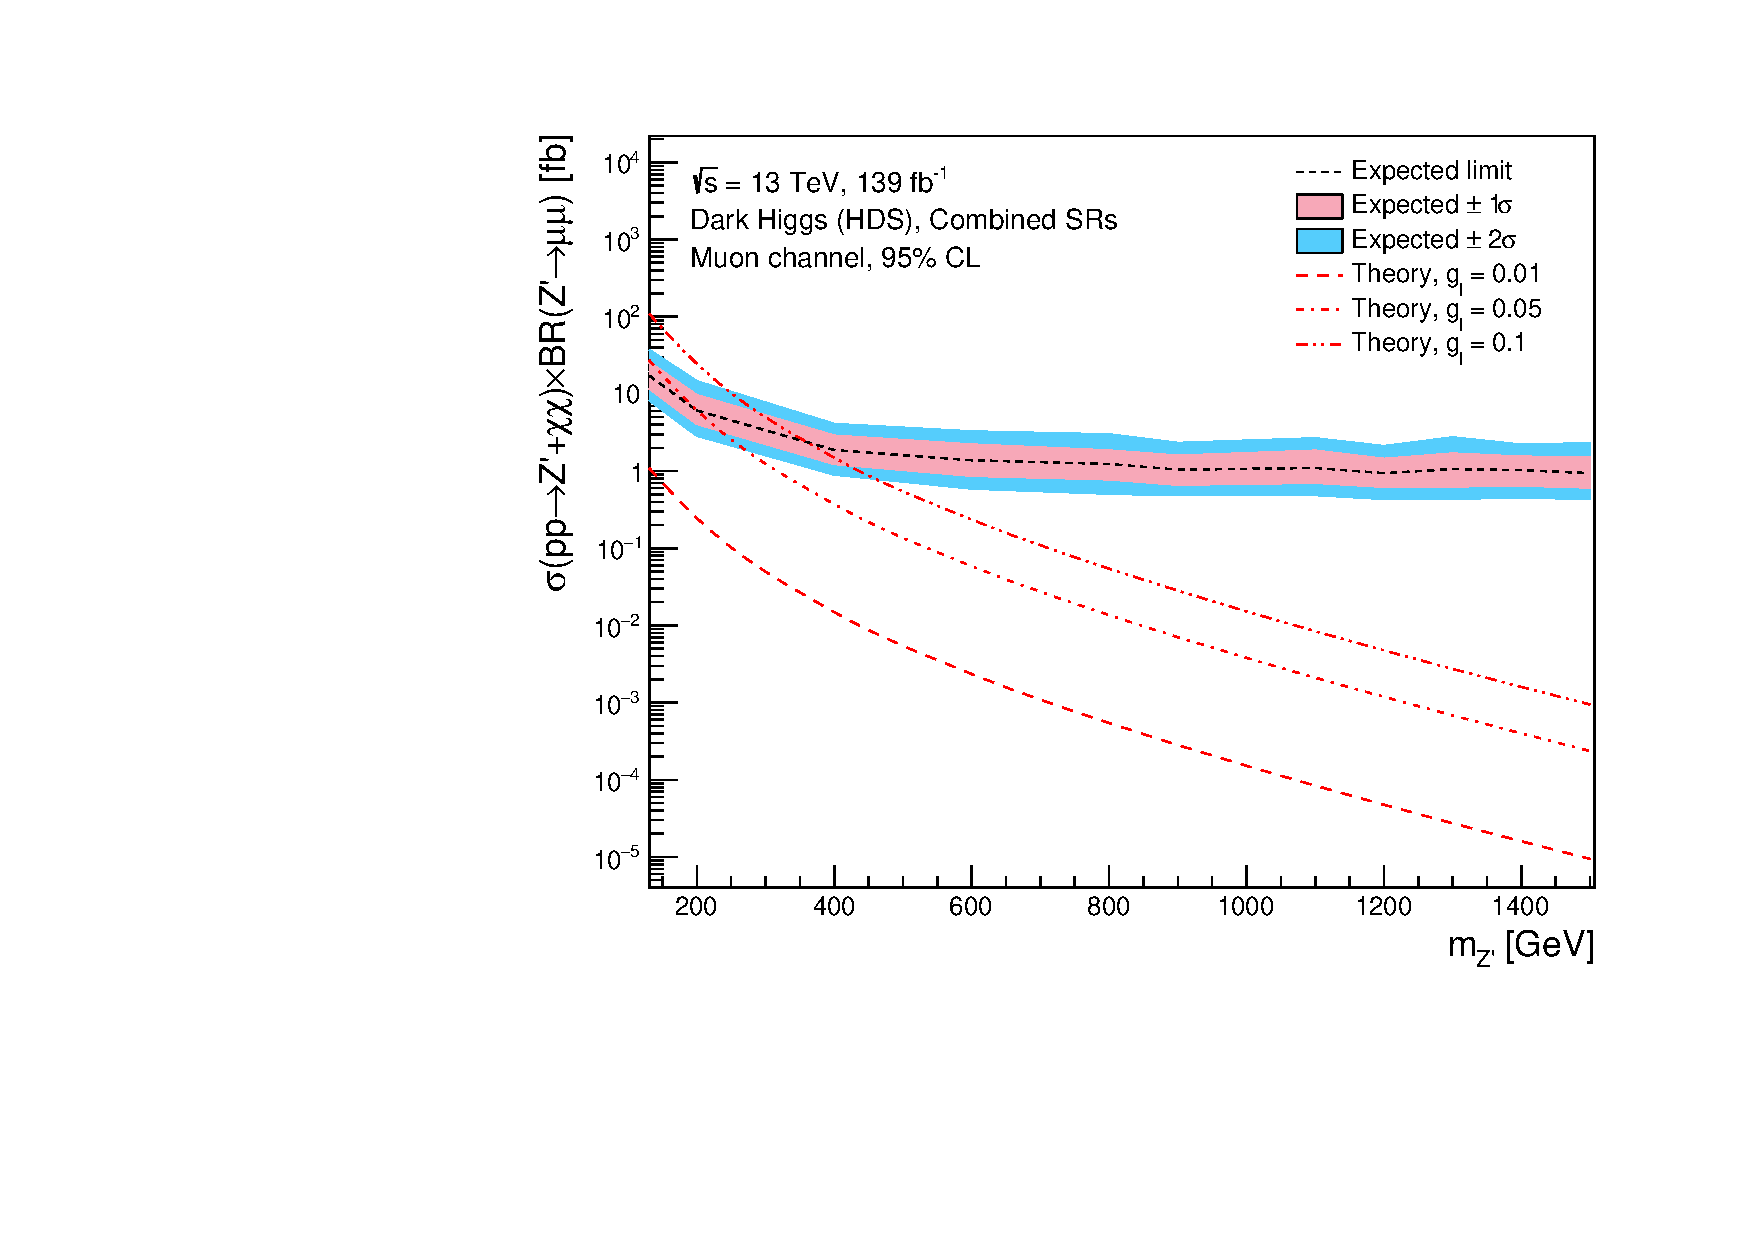
\includegraphics[width=1\textwidth]{Limits/Model_independent/DH_HDS/mass_exclusion_uu.pdf}
   \end{subfigure}
   \caption{Mass exclusion limits results for DH HDS model on $ee$ and $\mu\mu$ channel in combined SRs}\label{fig:DH_HDS_me_comb}
\end{figure}
Even further, we can statistically combine both of these results to get the exclusion on a general dilepton final state. Following this method for all other five models we can get the results in Figure \ref{fig:model_indep_exclusions}.\\
\\Where again we assumed that we have the same efficiency and number of background events on the last bin when increasing the lepton coupling constant.

\clearpage
\section{Mass exclusion limits for the combined channels}
\begin{figure}[!ht]
	\centering
	\begin{subfigure}[b]{0.49\textwidth}
      \centering
      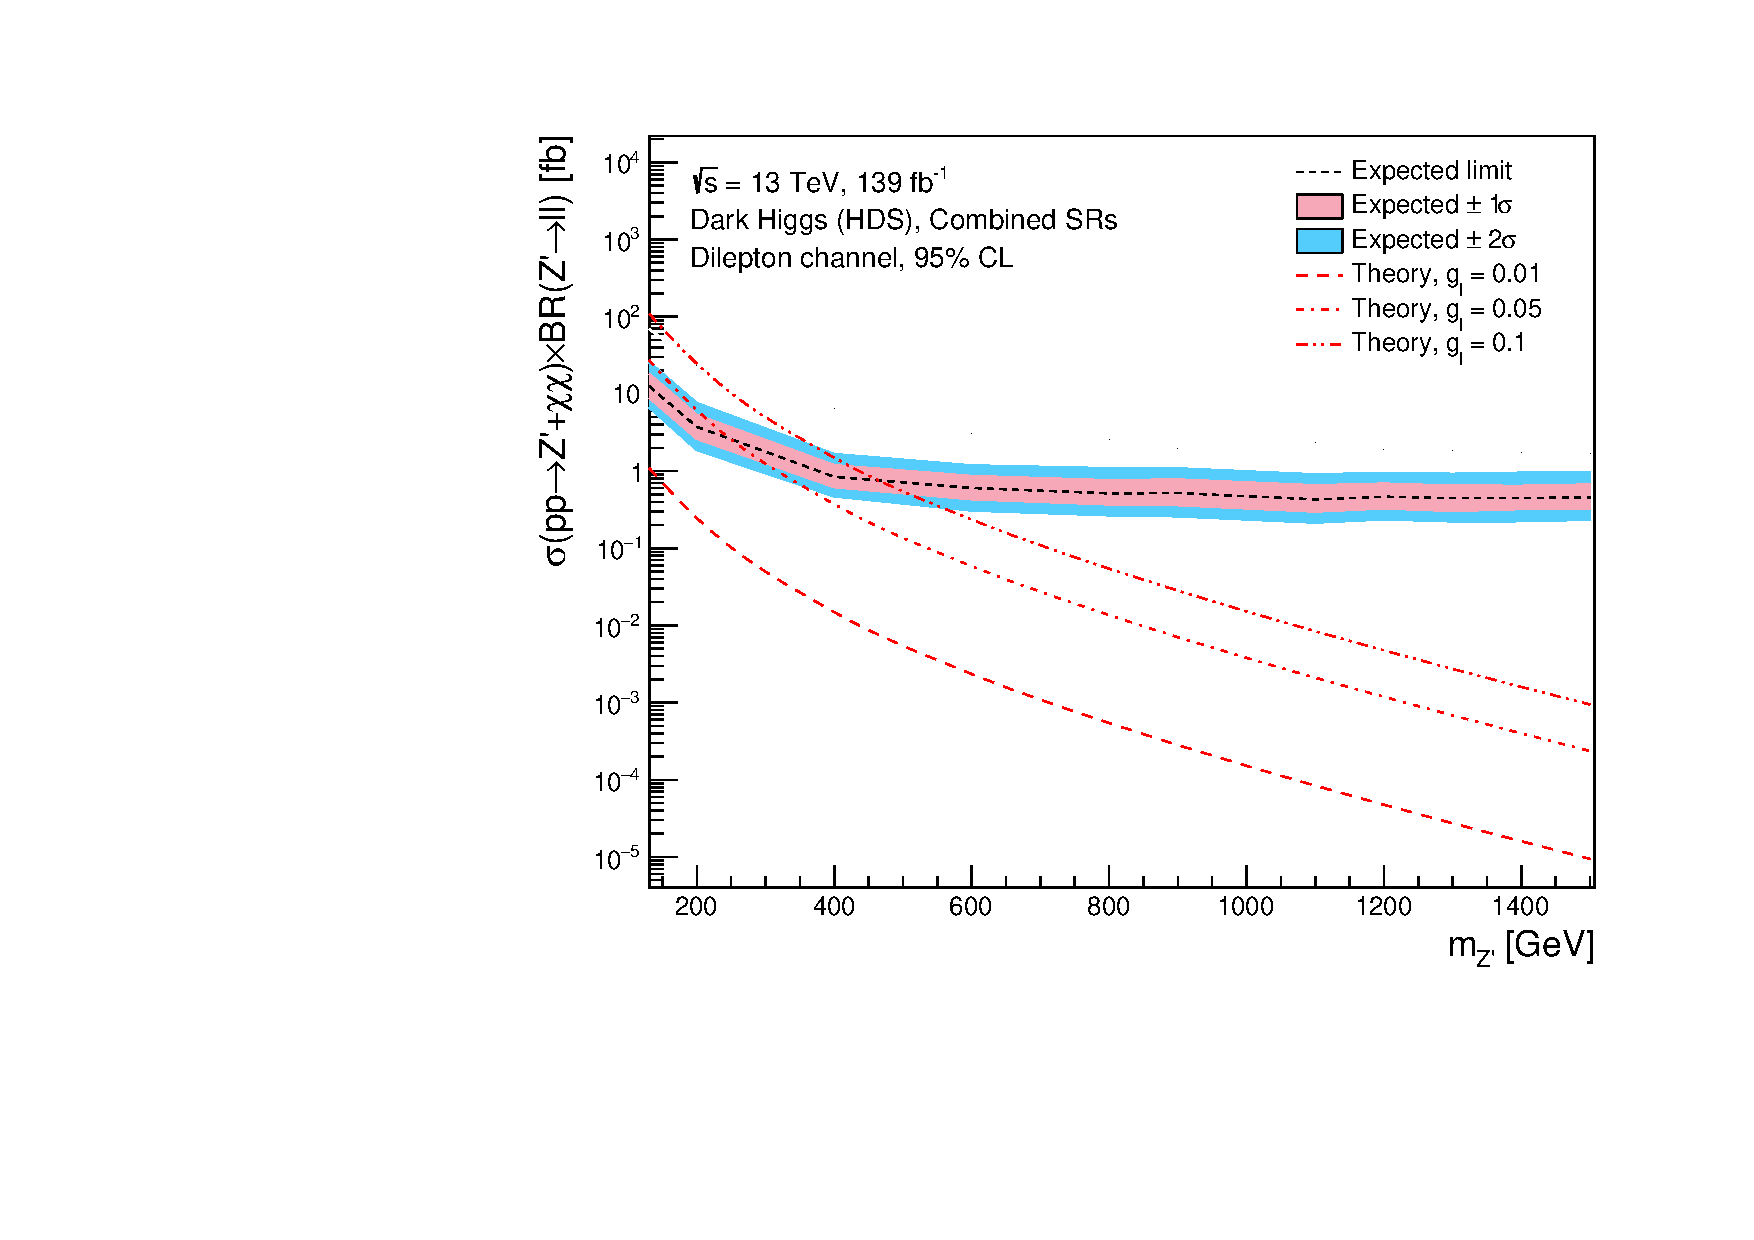
\includegraphics[width=1\textwidth]{Limits/Model_independent/DH_HDS/mass_exclusion_comb.pdf}
   \end{subfigure}
   \hfill
   \begin{subfigure}[b]{0.49\textwidth}
      \centering
      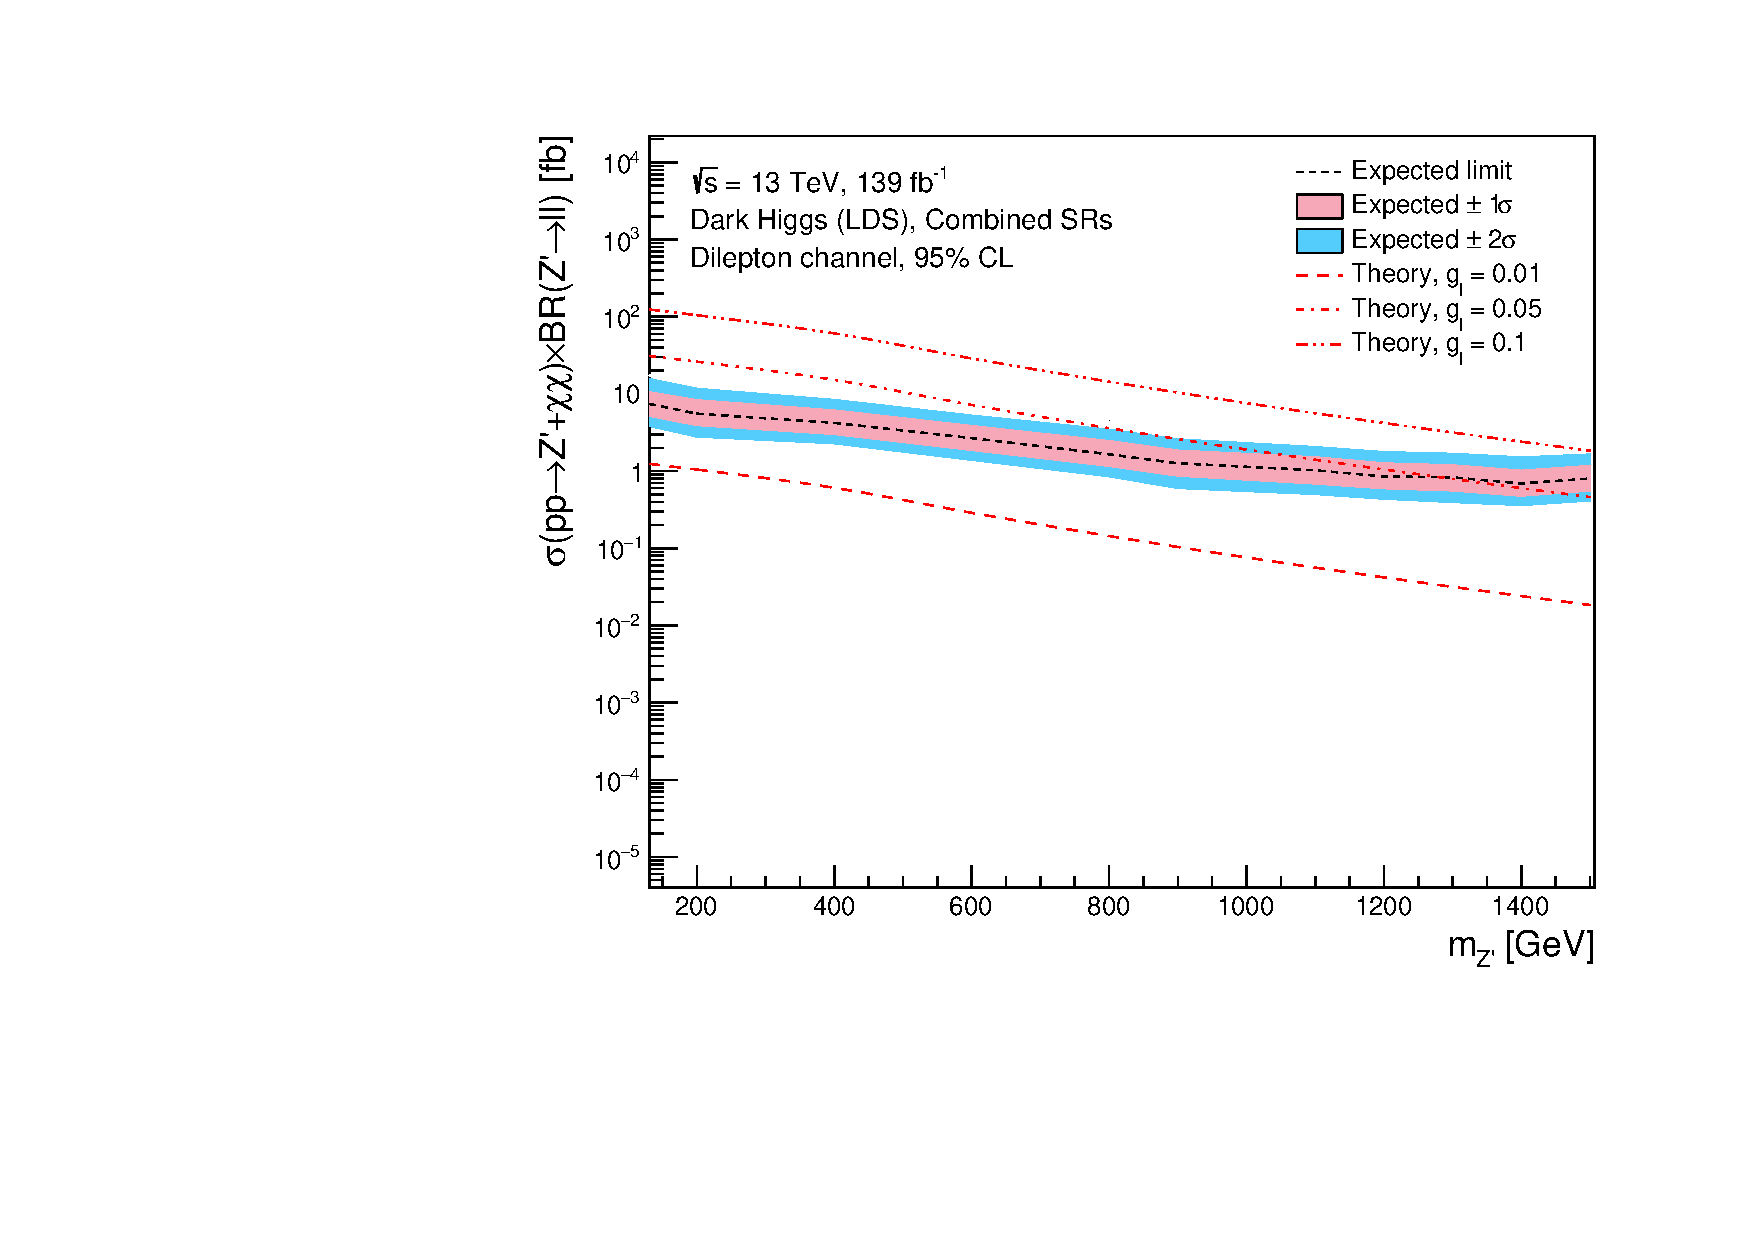
\includegraphics[width=1\textwidth]{Limits/Model_independent/DH_LDS/mass_exclusion_comb.pdf}
   \end{subfigure}
   \hfill
   \begin{subfigure}[b]{0.49\textwidth}
      \centering
      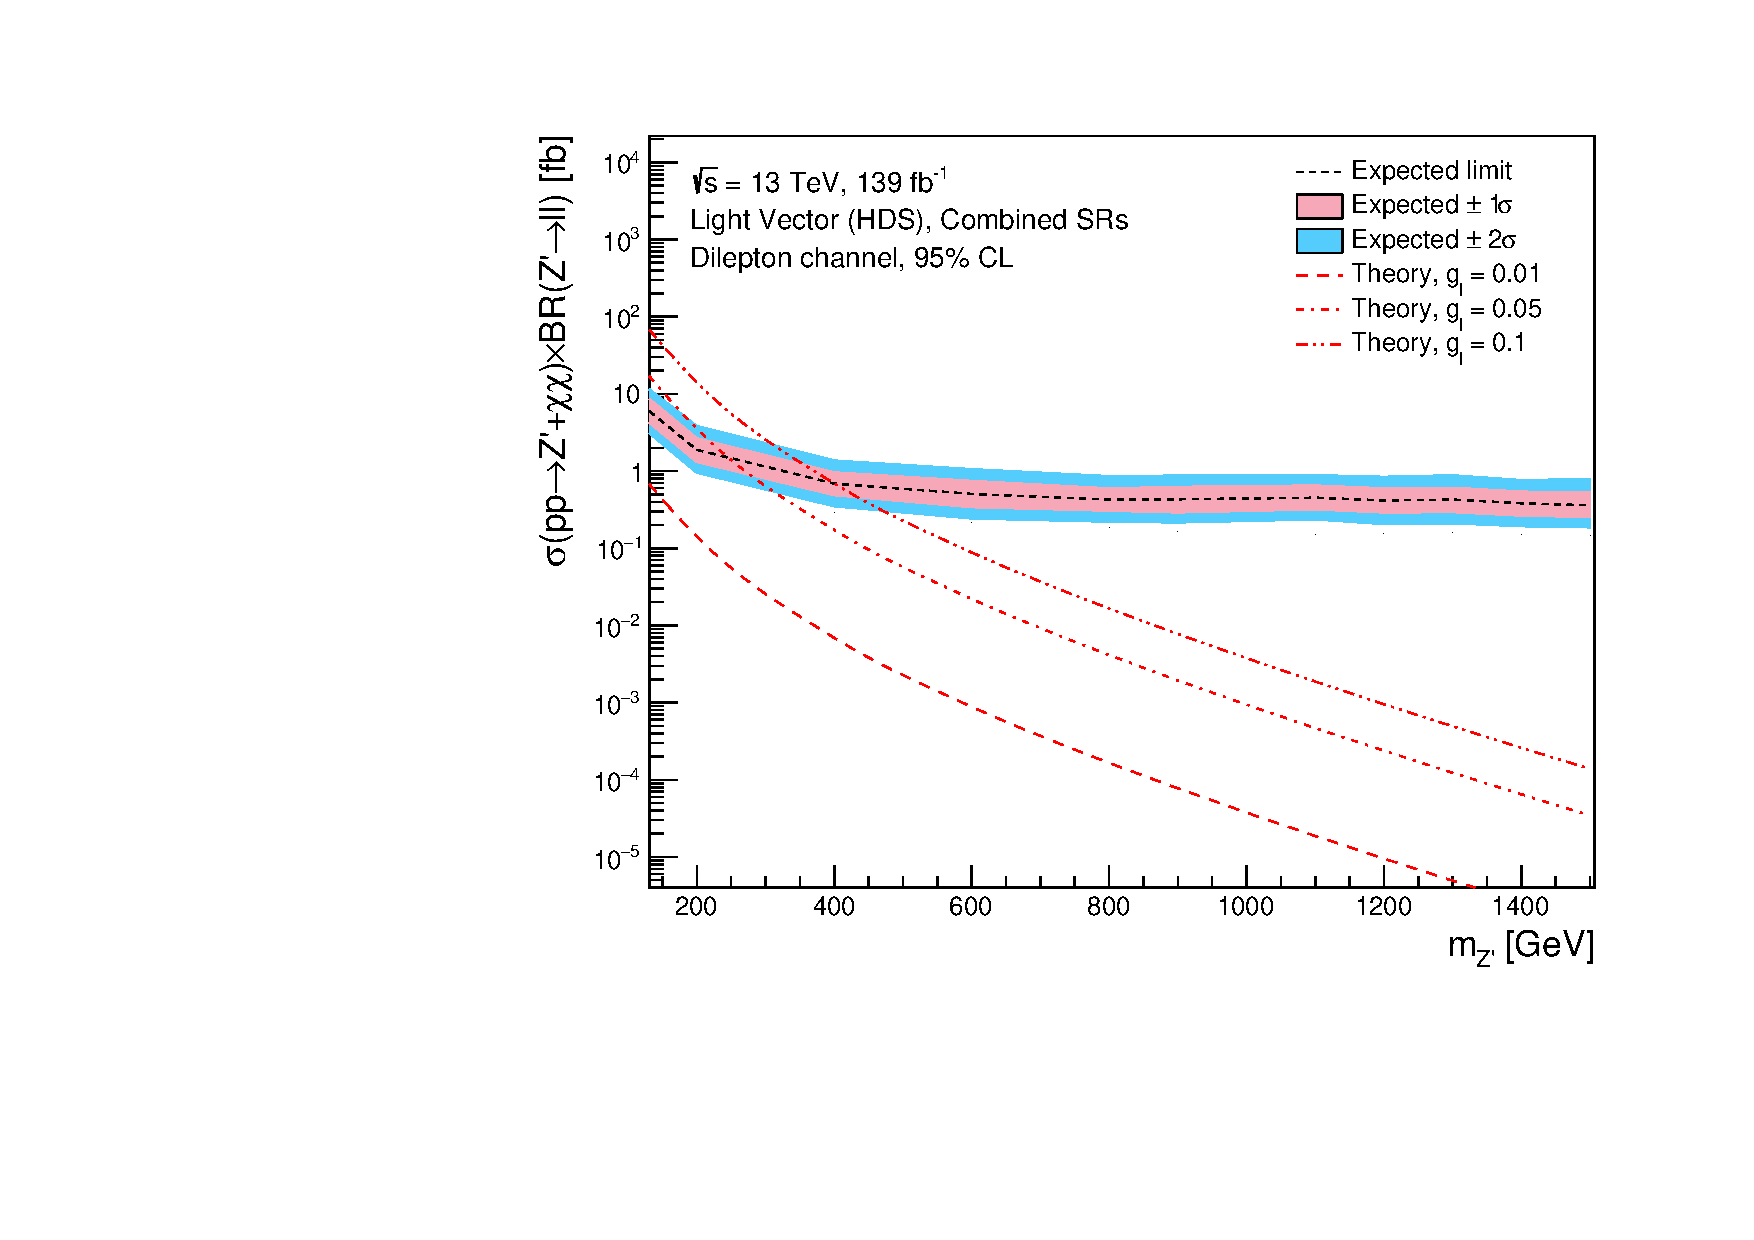
\includegraphics[width=1\textwidth]{Limits/Model_independent/LV_HDS/mass_exclusion_comb.pdf}
   \end{subfigure}
   \hfill
   \begin{subfigure}[b]{0.49\textwidth}
      \centering
      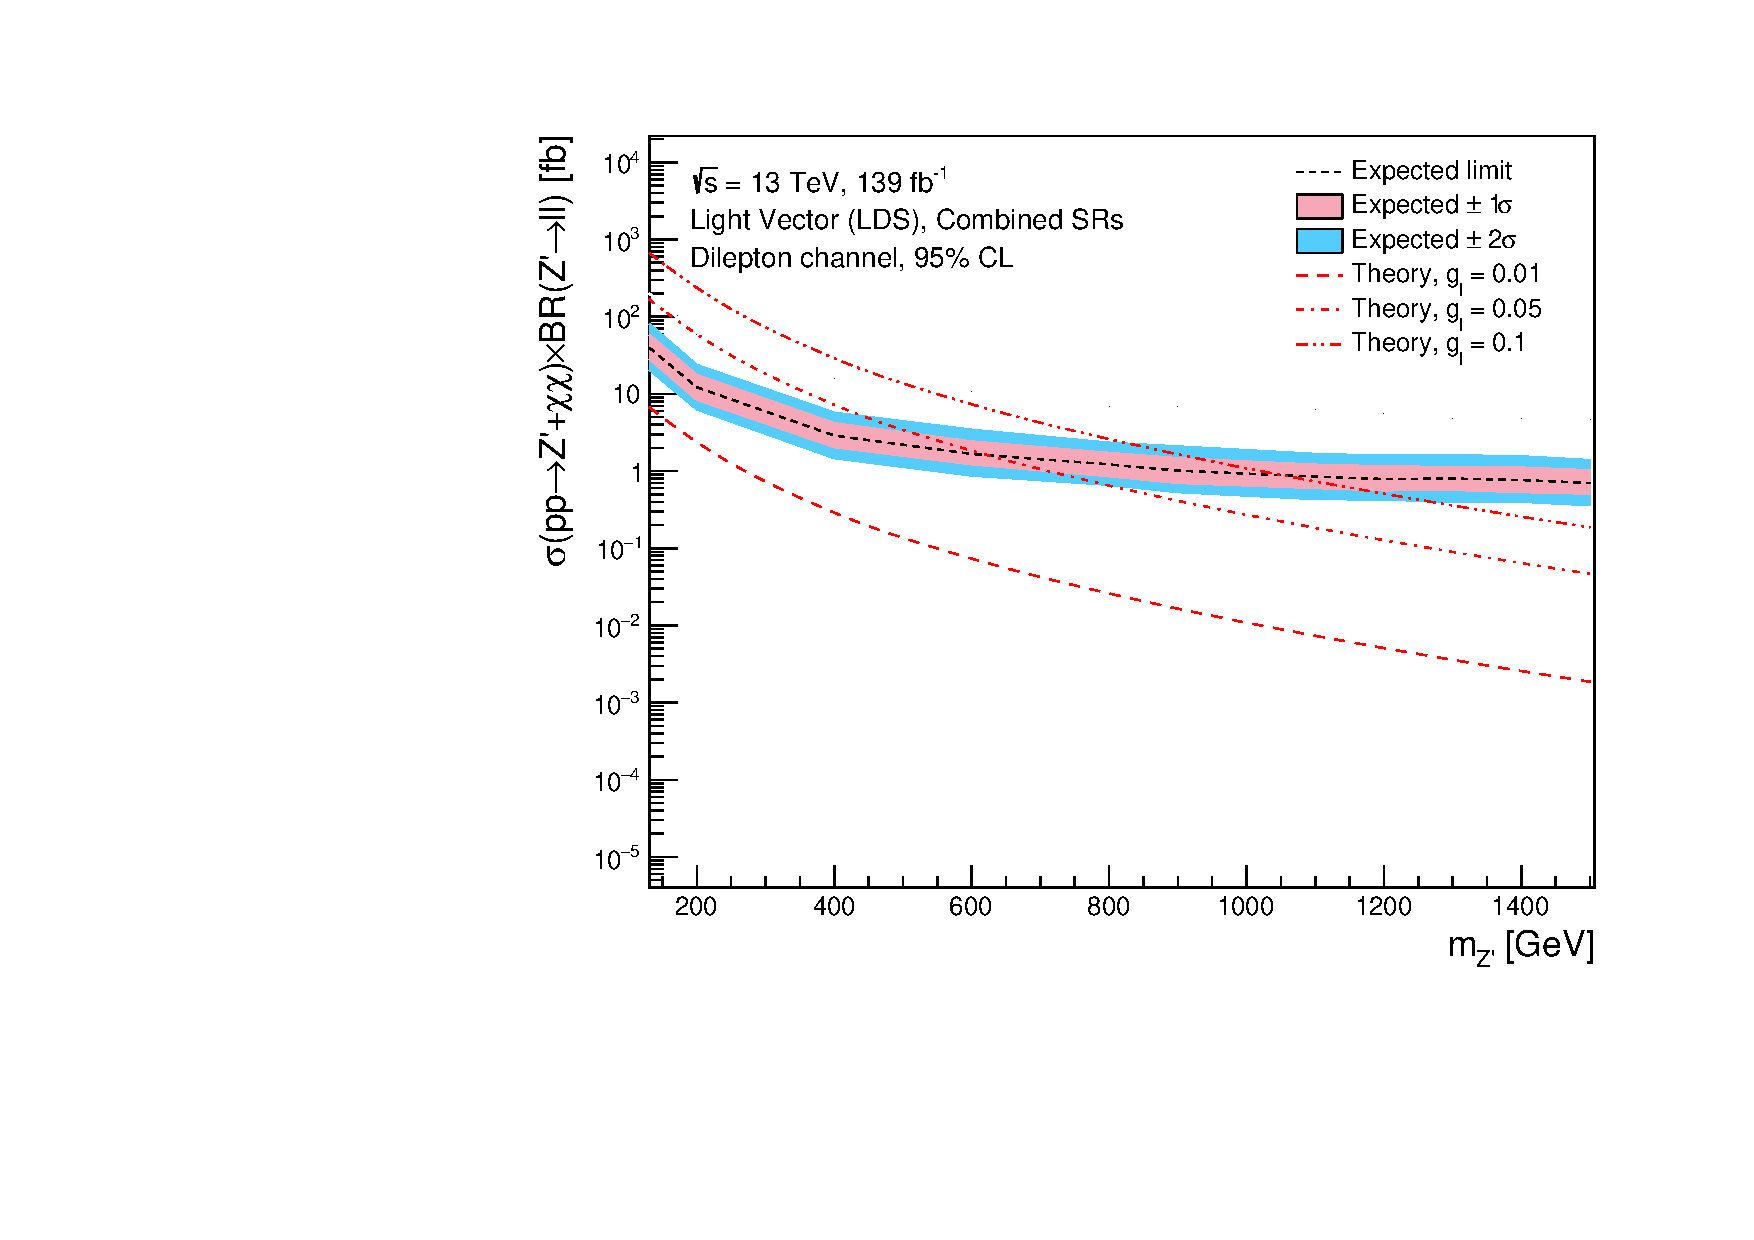
\includegraphics[width=1\textwidth]{Limits/Model_independent/LV_LDS/mass_exclusion_comb.pdf}
   \end{subfigure}
   \hfill
	\begin{subfigure}[b]{0.49\textwidth}
      \centering
      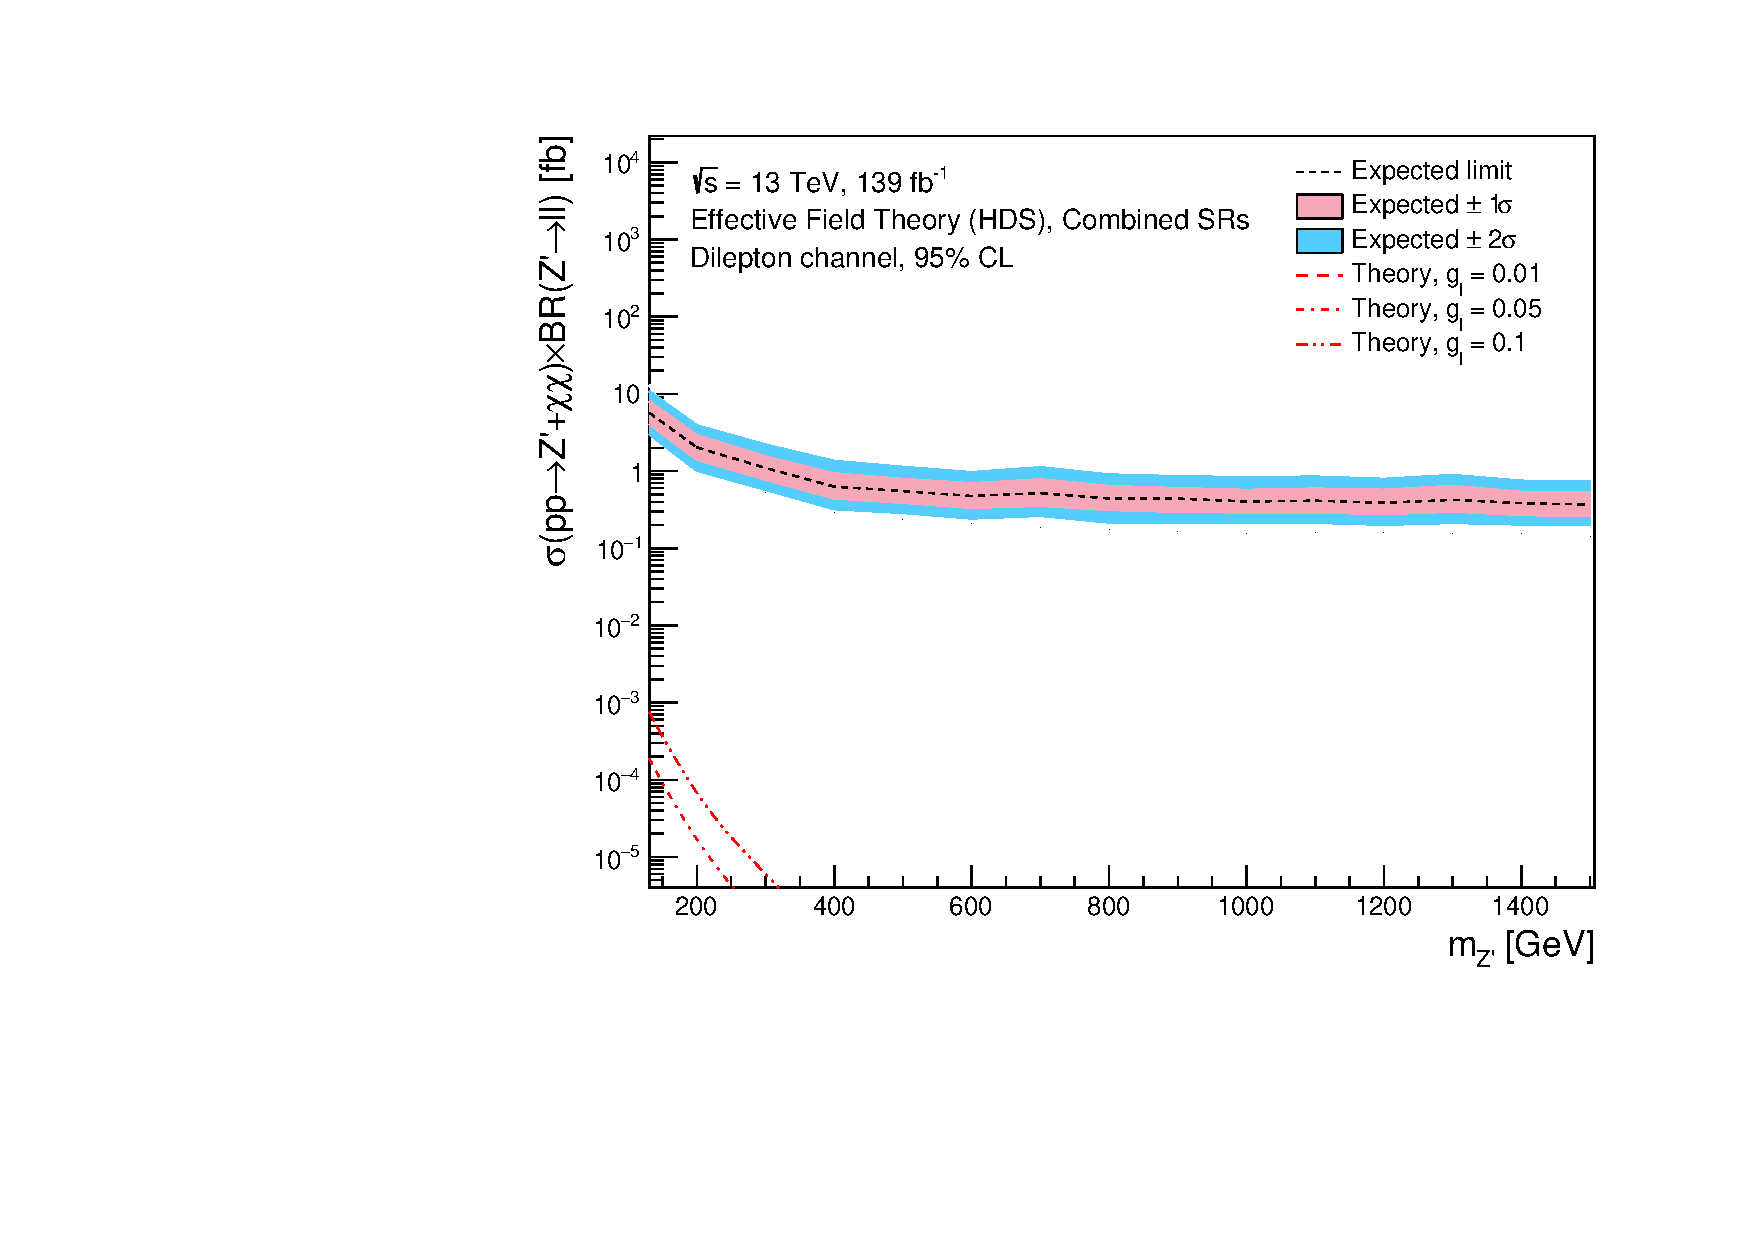
\includegraphics[width=1\textwidth]{Limits/Model_independent/EFT_HDS/mass_exclusion_comb.pdf}
   \end{subfigure}
   \hfill
   \begin{subfigure}[b]{0.49\textwidth}
      \centering
      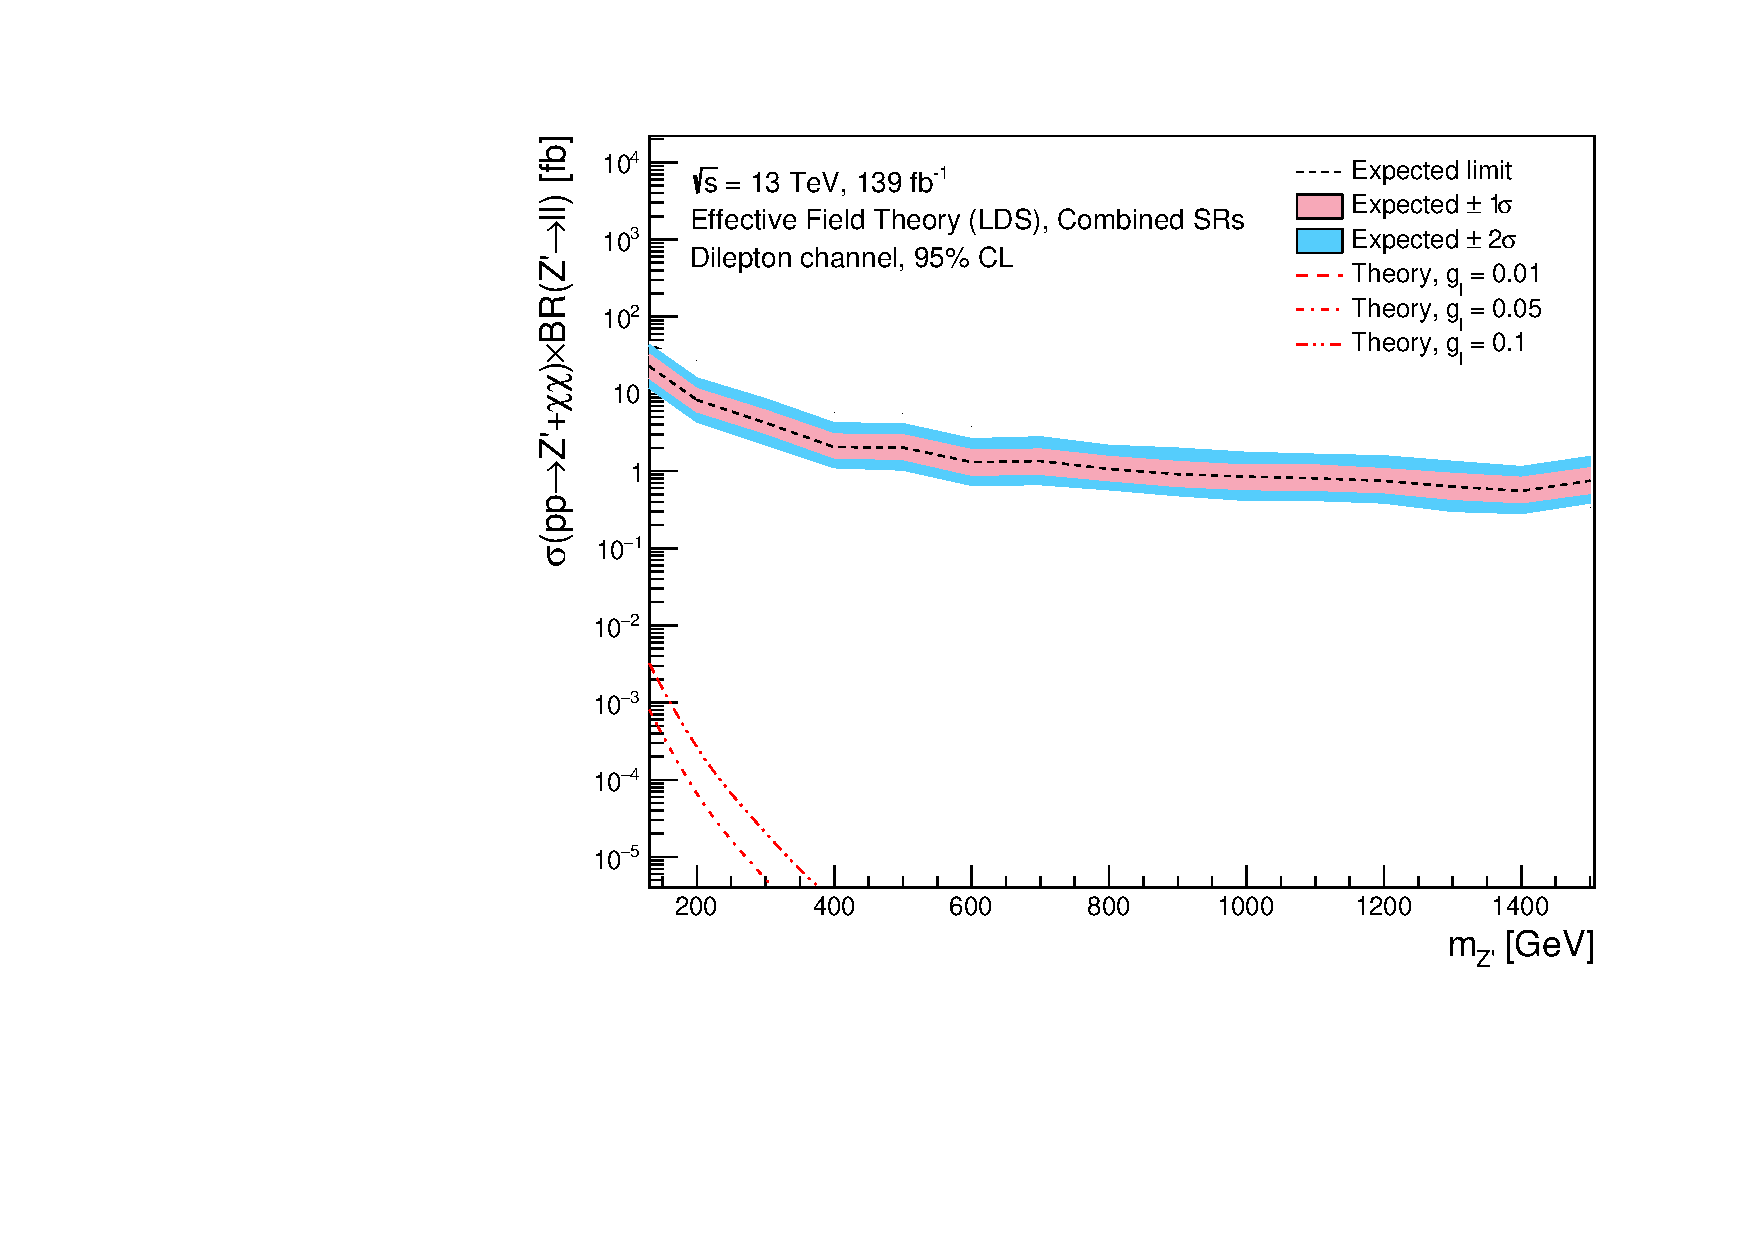
\includegraphics[width=1\textwidth]{Limits/Model_independent/EFT_LDS/mass_exclusion_comb.pdf}
   \end{subfigure}
   \caption[Mass exclusion limits of combined $ee$ and $\mu\mu$ channel for all models]{Mass exclusion limits of combined $ee$ and $\mu\mu$ channel for all models}\label{fig:model_indep_exclusions}
\end{figure}
\clearpage

\end{document}